\documentclass[11pt]{report}
% Style of the course's own documents (organisation/src/preamble.tex),
% extended for a handbook: listings, figures, a few boxes.
\usepackage[a4paper,margin=2.3cm,headheight=14pt]{geometry}
\usepackage[T1]{fontenc}
\usepackage[utf8]{inputenc}
\usepackage{lmodern}
\usepackage{microtype}
\usepackage{booktabs}
\usepackage{longtable}
\usepackage{array}
\usepackage{xcolor}
\usepackage{enumitem}
\usepackage{amssymb}
\usepackage{amsmath}
\usepackage{fancyhdr}
\usepackage{listings}
\usepackage{tikz}
\usetikzlibrary{arrows.meta,positioning,calc,fit,shapes.geometric,decorations.pathreplacing}
\usepackage[hidelinks]{hyperref}

\definecolor{warnbg}{RGB}{255,247,230}
\definecolor{warnrule}{RGB}{204,136,0}
\definecolor{newbg}{RGB}{235,245,255}
\definecolor{newrule}{RGB}{40,110,190}
\definecolor{keybg}{RGB}{237,247,237}
\definecolor{keyrule}{RGB}{50,120,60}
\definecolor{headgray}{RGB}{90,90,90}
\definecolor{codebg}{RGB}{248,248,248}

\usepackage[most]{tcolorbox}

\newtcolorbox{warnbox}[1][]{colback=warnbg,colframe=warnrule,boxrule=0.8pt,
  left=6pt,right=6pt,top=5pt,bottom=5pt,arc=1pt,#1}
\newtcolorbox{infobox}[1][]{colback=newbg,colframe=newrule,boxrule=0.8pt,
  left=6pt,right=6pt,top=5pt,bottom=5pt,arc=1pt,#1}
% "In SWEB": where the idea shows up in the course's kernel
\newtcolorbox{swebbox}[1][]{colback=newbg,colframe=newrule,boxrule=0.8pt,
  left=6pt,right=6pt,top=5pt,bottom=5pt,arc=1pt,
  title={In SWEB},fonttitle=\bfseries\small,coltitle=white,colbacktitle=newrule,#1}
% end-of-chapter summary
\newtcolorbox{keybox}[1][]{colback=keybg,colframe=keyrule,boxrule=0.8pt,
  left=6pt,right=6pt,top=5pt,bottom=5pt,arc=1pt,
  title={Key points},fonttitle=\bfseries\small,coltitle=white,colbacktitle=keyrule,#1}

\newcommand{\tbd}{\textcolor{warnrule}{\textbf{[confirm]}}}
\newcommand{\code}[1]{\texttt{#1}}
\newcommand{\file}[1]{\texttt{\small #1}}
\newcommand{\module}[1]{\textsf{module~#1}}

\setlist[itemize]{topsep=2pt,itemsep=1.5pt,parsep=0pt,leftmargin=1.3em}
\setlist[enumerate]{topsep=2pt,itemsep=1.5pt,parsep=0pt,leftmargin=1.6em}
\setlist[description]{topsep=2pt,itemsep=1.5pt,parsep=0pt,leftmargin=1.3em}

\newcolumntype{L}[1]{>{\raggedright\arraybackslash}p{#1}}

\lstset{
  language=C,
  basicstyle=\ttfamily\small,
  keywordstyle=\color{newrule}\bfseries,
  commentstyle=\color{headgray}\itshape,
  stringstyle=\color{warnrule!80!black},
  backgroundcolor=\color{codebg},
  frame=single, rulecolor=\color{black!15}, framesep=3pt,
  xleftmargin=4pt, xrightmargin=4pt, aboveskip=6pt, belowskip=4pt,
  columns=fullflexible, keepspaces=true, showstringspaces=false,
  upquote=true, tabsize=2,
  morekeywords={size_t,ssize_t,pid_t,pthread_t,pthread_mutex_t,pthread_cond_t,
                sem_t,uint8_t,uint32_t,uint64_t,bool,_Atomic,atomic_int,
                atomic_flag,__thread,_Noreturn,__asm__,volatile,pointer,uint64}
}
\lstdefinestyle{shell}{language=bash,morekeywords={},keywordstyle=\color{black}}
\lstdefinestyle{cpp}{language=C++}

\pagestyle{fancy}
\fancyhf{}
\renewcommand{\headrulewidth}{0.4pt}
\fancyhead[L]{\small\textcolor{headgray}{OS preparation handbook}}
\fancyhead[R]{\small\textcolor{headgray}{\leftmark}}
\fancyfoot[C]{\small\thepage}
\renewcommand{\chaptermark}[1]{\markboth{\thechapter\ \ #1}{}}
\fancypagestyle{plain}{\fancyhf{}\renewcommand{\headrulewidth}{0pt}\fancyfoot[C]{\small\thepage}}

\renewcommand{\arraystretch}{1.25}
\setlength{\parskip}{3pt}
\setlength{\parindent}{0pt}
\setlength{\emergencystretch}{3em}   % fewer overfull lines with long \code words


\begin{document}

\begin{titlepage}
  \centering
  \vspace*{3cm}
  {\Huge\bfseries Operating Systems\\[6pt] Preparation Handbook\par}
  \vspace{1cm}
  {\Large Threads, synchronisation, system calls, memory, scheduling ---\\
   and how they meet in SWEB\par}
  \vspace{2cm}
  {\large Companion to the twelve modules in \texttt{preparations/}\par}
  \vfill
  \begin{infobox}
  Every chapter belongs to the module with the same number: read the
  chapter, run the module's examples, then do its assignment. The boxes
  titled \emph{In SWEB} point to the place in the course's kernel where the
  idea turns into code you will change for A1.
  \end{infobox}
  \vspace{1cm}
  {\small A self-study companion for Operating Systems at TU Graz,\\ winter semester 2026/27 --- not official course material\par}
\end{titlepage}

\tableofcontents

\setcounter{chapter}{-1}
\chapter{The C toolbox}
\label{ch:c}

Operating-systems code is C (or, in SWEB, a careful subset of C++) with no
safety net: no garbage collector, no bounds checks, no exceptions. Most
bugs you will hunt in A1 are pointer and lifetime bugs that corrupt memory
silently and crash much later, somewhere else. This chapter is the minimum
toolkit: how to build with the right flags, how to let the compiler's
sanitizers find those bugs for you, and the three C ideas every later
chapter relies on --- pointers, lifetimes, and function pointers.

\section{Toolchain: from source to a running program}

\begin{lstlisting}[style=shell]
gcc -std=gnu17 -Wall -Wextra -g -O1 -fsanitize=address,undefined prog.c -o prog
\end{lstlisting}

\begin{description}
  \item[\code{-Wall -Wextra}] turn on the warnings that catch real bugs
    (unused results, sign mix-ups, missing returns). Treat a warning as a
    bug report you have not read yet. The course modules also turn a few
    warnings into errors, e.g.\ \code{-Werror=implicit-function-declaration}:
    calling a function without a prototype silently truncates pointers to
    \code{int} on 64-bit machines.
  \item[\code{-g}] debug information: line numbers in sanitizer reports
    and in \code{gdb}.
  \item[\code{-O0/-O1/-O2}] optimisation. Race bugs and missing
    \code{volatile}s often appear only at \code{-O2}, because the compiler
    then keeps values in registers and reorders memory accesses. The
    modules therefore test both a sanitizer build and an optimised build.
\end{description}

\code{make} rebuilds only what changed. Every module has a
\code{Makefile} with the targets \code{run} (examples) and \code{test}
(assignment). \code{make test IMPL=../../solutions/NN-...} builds the tests
against the reference solution instead of your own files.

\section{Sanitizers: let the compiler find your bugs}

A sanitizer is compiler instrumentation plus a run-time library. The
instrumented program checks every memory access (or every thread
interaction) and prints a report at the \emph{first} violation --- not at
the crash three functions later.

\begin{center}
\begin{tabular}{L{3.3cm}L{4.4cm}L{6.1cm}}
\toprule
\textbf{Sanitizer} & \textbf{Flag} & \textbf{Finds} \\
\midrule
AddressSanitizer & \code{-fsanitize=address} & out-of-bounds accesses (heap,
stack, globals), use after free, use after return, double free, leaks \\
Undefined\-Behavior\-Sanitizer & \code{-fsanitize=undefined} & signed overflow,
bad shifts, misaligned pointers, NULL dereference, out-of-range enum values \\
ThreadSanitizer & \code{-fsanitize=thread} & data races (chapter~3),
lock-order inversions (chapter~6) \\
\bottomrule
\end{tabular}
\end{center}

Reading a report: the first lines name the \emph{kind} of error
(\code{heap-use-after-free}, \code{stack-buffer-overflow}, \dots) and the
access; then come three stack traces --- where the bad access happened,
where the memory was allocated, and where it was freed. Start at the
first frame that is in your code.

\begin{warnbox}
ASan and TSan cannot be combined (they instrument memory differently),
and ThreadSanitizer fails on recent kernels with high address-space
randomisation (\emph{``unexpected memory mapping''}). The modules' test
runner starts TSan binaries under \code{setarch -R}, which disables
randomisation for that one process.
\end{warnbox}

\section{Pointers}

A pointer is an address plus a type. The type says how many bytes
\code{*p} reads and how far \code{p + 1} moves.

\begin{lstlisting}
int a[4] = {1, 2, 3, 4};
int *p = a;            /* an array decays to a pointer to its first element */
p + 2;                 /* address of a[2]: moves by 2 * sizeof(int) bytes    */
*(p + 2) == p[2];      /* identical: indexing is pointer arithmetic          */
sizeof a;              /* 16: the array; sizeof p would be 8: the pointer    */
\end{lstlisting}

\paragraph{Out-parameters.} C returns one value. A function that must
produce more writes through pointers the caller passes in ---
\code{pthread\_create(\&tid, ...)} stores the new thread's id in the
caller's variable, and every system call that reads data does the same
with a buffer.

\paragraph{\code{void *}.} A pointer to ``something''. It converts to and
from any object pointer without a cast in C, but cannot be dereferenced
or used in arithmetic until it is converted back to a real type. Generic
code (\code{qsort}, \code{pthread\_create}, a thread library's argument)
passes \code{void *} and trusts the caller to know the real type.

\paragraph{Integers as pointers.} Kernels constantly convert between
pointers and integers: a system call receives user pointers as plain
numbers in registers (SWEB: \code{size\_t}, or its \code{pointer} type).
\code{uintptr\_t}/\code{size\_t} are wide enough; \code{int} is not. This
is also why a \emph{number} chosen by a user must be validated before the
kernel treats it as an address (chapter~7).

\section{Lifetimes: stack, heap, static}

\begin{center}
\begin{tabular}{L{2.2cm}L{4.4cm}L{7.2cm}}
\toprule
\textbf{Storage} & \textbf{Lives} & \textbf{Typical bug} \\
\midrule
stack (locals) & until the function returns & returning or storing the
address of a local; a thread using a pointer to its creator's local after
the creator returned \\
heap (\code{malloc}) & until \code{free} & use after free, double free,
leak (never freed) \\
static (globals, \code{static}) & the whole program & shared between all
threads: needs synchronisation (chapter~3) \\
\bottomrule
\end{tabular}
\end{center}

The stack is the dangerous one for thread code: a loop that passes
\code{\&i} to every new thread passes the \emph{same} address, which keeps
changing --- and may no longer exist when the thread reads it
(\module{02}, \file{bug1\_loop\_index.c} and \file{bug2\_dead\_arguments.c}).

\begin{lstlisting}
int *broken(void) {
  int x = 42;
  return &x;        /* x dies here: the caller gets a dangling pointer */
}
\end{lstlisting}

AddressSanitizer reports this as \code{stack-use-after-return} (with
\code{detect\_stack\_use\_after\_return=1}, which the modules set).

\section{Function pointers and callbacks}

A function's name, used without parentheses, is its address. A function
pointer stores such an address and calls through it:

\begin{lstlisting}
int twice(int x) { return 2 * x; }
int (*f)(int) = twice;           /* pointer to function taking int, returning int */
f(21);                           /* 42 */
\end{lstlisting}

\paragraph{The callback pattern: function + context.} A library that
calls back into your code cannot know what data your code needs, so it
takes a function pointer \emph{and} an opaque \code{void *} that it hands
back unchanged:

\begin{lstlisting}
int pthread_create(pthread_t *thread, const pthread_attr_t *attr,
                   void *(*start_routine)(void *), void *arg);
\end{lstlisting}

\code{start\_routine} is ``what to run'', \code{arg} is ``with what''. The
library never looks inside \code{arg} --- which is also why the SWEB
kernel must \emph{not} validate it as a pointer (chapter~7): it may just
as well be the number 7 cast to \code{void *}. Returning a value works the
same way backwards: \code{start\_routine} returns a \code{void *} that
\code{pthread\_join} hands to the joiner.

\begin{swebbox}
SWEB is written in C++, but kernel C++: no exceptions, no standard
library (it brings its own \code{ustl} containers), fixed-width types
(\code{uint32}, \code{size\_t}, \code{pointer} for addresses). User
programs in \file{userspace/tests/} are plain C against SWEB's own small
libc (\file{userspace/libc}); the \code{pthread\_*} functions there are
empty stubs you will fill in.
\end{swebbox}

\begin{keybox}
\begin{itemize}
  \item Build with warnings on, and test with sanitizers \emph{and} with
    optimisation.
  \item Read a sanitizer report from the top: kind of error, bad access,
    allocation site, free site.
  \item Know where every object lives and how long; never hand a pointer
    to a local to code that outlives the function.
  \item Callbacks come as \emph{function pointer + opaque context}; the
    library never interprets the context.
\end{itemize}
\end{keybox}

\chapter{Processes}
\label{ch:processes}

A \emph{program} is a file. A \emph{process} is a program being executed:
an address space with code and data in it, at least one thread of
execution, and a set of resources the kernel keeps on its behalf (open
files, the current directory, a process id). This chapter looks at
processes from the outside --- through the system calls that create,
replace, wait for and signal them. Team F implements \code{fork} and
\code{exec} in SWEB for A1; Team P needs the same picture, because a
thread lives \emph{inside} a process.

\section{What the kernel keeps per process}

For every process the kernel has a record --- textbooks call it the
\emph{process control block} (PCB):

\begin{itemize}
  \item identity: process id (PID), parent PID, user id;
  \item the address space: page tables and the list of mapped regions;
  \item open files: the file-descriptor table;
  \item the current working directory, signal handlers, exit status;
  \item one or more threads, each with its own saved registers, stack and
    scheduling state (chapter~2).
\end{itemize}

The last point is exactly what SWEB does not have yet: there, a process
\emph{is} a thread (\code{class UserProcess : public Thread}), and the
first thing your group does in A1 (``Phase 0'') is to split the two.

\section{The address space}

Every process sees its own, private range of virtual addresses
(chapter~8 explains how the hardware makes that possible). On x86-64
Linux the lower half belongs to the process, the upper half to the
kernel (figure~\ref{fig:layout}).

\begin{figure}[htbp]
\centering
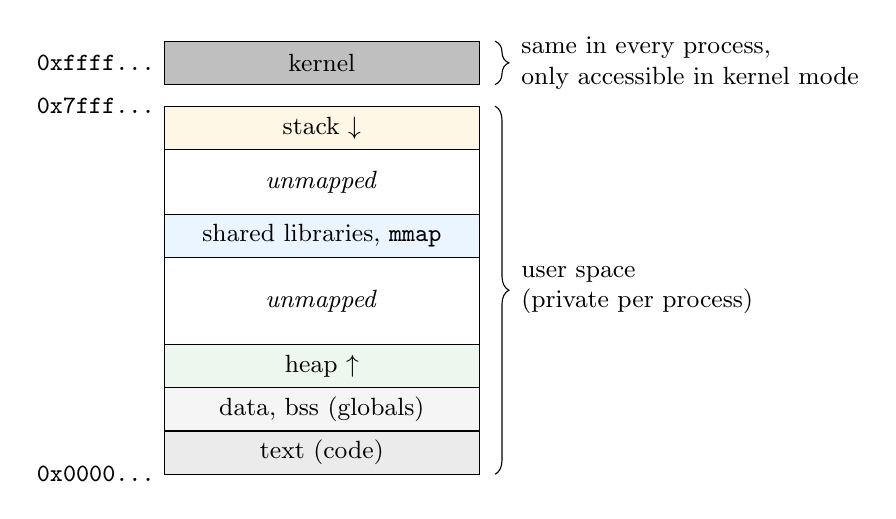
\begin{tikzpicture}[x=1cm,y=0.55cm,font=\small]
  \def\w{4}
  \draw[fill=black!8] (0,0) rectangle (\w,1) node[midway] {text (code)};
  \draw[fill=black!4] (0,1) rectangle (\w,2) node[midway] {data, bss (globals)};
  \draw[fill=keybg] (0,2) rectangle (\w,3) node[midway] {heap $\uparrow$};
  \draw (0,3) rectangle (\w,5) node[midway] {\emph{unmapped}};
  \draw[fill=newbg] (0,5) rectangle (\w,6) node[midway] {shared libraries, \code{mmap}};
  \draw (0,6) rectangle (\w,7.5) node[midway] {\emph{unmapped}};
  \draw[fill=warnbg] (0,7.5) rectangle (\w,8.5) node[midway] {stack $\downarrow$};
  \draw[fill=black!25] (0,9) rectangle (\w,10) node[midway] {kernel};
  \node[left] at (0,0) {\code{0x0000\dots}};
  \node[left] at (0,8.5) {\code{0x7fff\dots}};
  \node[left] at (0,9.5) {\code{0xffff\dots}};
  \draw[decorate,decoration={brace,amplitude=5pt}] (\w+0.2,8.5) -- (\w+0.2,0)
     node[midway,right=6pt,align=left] {user space\\(private per process)};
  \draw[decorate,decoration={brace,amplitude=5pt}] (\w+0.2,10) -- (\w+0.2,9)
     node[midway,right=6pt,align=left] {same in every process,\\only accessible in kernel mode};
\end{tikzpicture}
\caption{The address space of a process on x86-64 Linux (not to scale).}
\label{fig:layout}
\end{figure}

The heap grows upwards (\code{malloc} asks the kernel for more with
\code{brk}/\code{mmap}), the stack downwards. \file{/proc/<pid>/maps}
shows the real layout of a running process (\module{08}'s
\code{demand\_paging} example prints it).

\begin{swebbox}
The boundary is \code{USER\_BREAK} (\file{arch/x86/64/include/offsets.h}):
\code{0x0000800000000000}. A new SWEB process gets exactly one stack page,
the last page below \code{USER\_BREAK}, and its stack pointer starts at
\code{USER\_BREAK - 8}. Code and data are \emph{not} loaded up front: each
first access page-faults and \code{Loader::loadPage} copies the page from
the binary (chapter~8).
\end{swebbox}

\section{fork, exec, wait, exit}

\paragraph{\code{fork()}} creates a copy of the calling process: same code,
a copy of all memory, copies of the file descriptors (pointing to the
same open files). It is called once and \emph{returns twice} --- in the
parent with the child's PID, in the child with 0:

\begin{lstlisting}
pid_t pid = fork();
if (pid < 0)        { perror("fork"); }        /* no child */
else if (pid == 0)  { /* child */ }
else                { /* parent: pid = the child's PID */ }
\end{lstlisting}

``Returns twice'' is less magic than it sounds: the kernel copies the
parent's saved user registers into the child and then changes one of
them --- the return-value register (\code{rax} on x86-64) is 0 in the
child. When each of them is next scheduled, both continue at the
instruction after the system call. Copying all memory would be slow; real
kernels share the pages and copy a page only when one side writes to it
(\emph{copy-on-write}, chapter~8).

\paragraph{\code{exec*()}} replaces the program running in the current
process: new code, new data, new stack, same PID, same open file
descriptors (unless marked close-on-exec). On success it does not return
--- the code that called it no longer exists.

\paragraph{\code{exit(status)} and \code{wait}.} A process ends with an
exit status; its parent collects it with \code{wait}/\code{waitpid}:

\begin{lstlisting}
int status;
waitpid(pid, &status, 0);
if (WIFEXITED(status))        printf("exit code %d\n", WEXITSTATUS(status));
else if (WIFSIGNALED(status)) printf("killed by signal %d\n", WTERMSIG(status));
\end{lstlisting}

The shell does exactly this for every command: \code{fork}, \code{exec}
in the child, \code{waitpid} in the parent (\module{01}'s \code{minish}).

\paragraph{Zombies and orphans.} A process that has exited but whose
status has not been collected yet is a \emph{zombie}: its memory is gone,
but its PCB with the exit status must stay until the parent calls
\code{wait}. A process whose parent dies first is an \emph{orphan}; it is
adopted by \code{init} (PID~1), which reaps it. The same idea returns for
threads: a finished, not yet joined thread keeps its return value
(chapter~10).

\section{File descriptors and pipes}

A file descriptor is an index into the process's descriptor table; each
entry points to an \emph{open file} object in the kernel (position,
flags, the file or pipe itself). By convention 0, 1 and 2 are standard
input, output and error.

\begin{itemize}
  \item \code{fork} copies the table: parent and child share the same open
    files (and the same file position).
  \item \code{dup2(old, new)} makes \code{new} refer to the same open file
    as \code{old} --- this is how a shell redirects output.
  \item \code{pipe(fds)} creates a kernel buffer with a read end
    (\code{fds[0]}) and a write end (\code{fds[1]}). A reader blocks while
    the buffer is empty, a writer while it is full.
\end{itemize}

\begin{warnbox}
A reader sees end-of-file only when \emph{every} write end is closed ---
in every process. A forgotten write end in the parent keeps \code{wc}
waiting forever. Rule: after \code{fork} + \code{dup2}, close every pipe
end you do not use, in every process.
\end{warnbox}

\section{Signals}

A signal is an asynchronous notification to a process: \code{SIGINT}
(Ctrl-C), \code{SIGSEGV} (bad memory access), \code{SIGCHLD} (a child
changed state), \code{SIGALRM} (a timer expired), \code{SIGKILL} (cannot
be caught). Each has a default action (terminate, core dump, ignore,
stop); \code{sigaction} installs a handler instead.

A handler interrupts the program at an arbitrary instruction --- like a
hardware interrupt interrupts the kernel. Consequently a handler may only
call \emph{async-signal-safe} functions (\code{write}, \code{\_exit},
\dots, but not \code{printf} or \code{malloc}, which may hold internal
locks at the moment of interruption) and should communicate through a
\code{volatile sig\_atomic\_t} flag. Chapter~10 uses a timer signal to
preempt user-level threads and runs into exactly this rule.

\section{A trap: buffered output and fork}

\code{printf} does not write immediately: \code{stdio} collects output in
a buffer inside the process and flushes it at a newline (terminal),
when the buffer is full (pipe, file) or at exit. \code{fork} copies that
buffer too --- output that was ``printed'' before \code{fork} but not yet
flushed appears \emph{twice}, once from each process. Call
\code{fflush(stdout)} before \code{fork} (\module{01},
\code{stdio\_trap.c}; \module{08}'s \code{cow\_fork.c} fell into it while
being written).

\begin{swebbox}
Baseline SWEB has no \code{fork} and no \code{exec}: the shell starts
programs with the course's own \code{createprocess} system call
(\file{common/source/kernel/Syscall.cpp}), which creates a new
\code{UserProcess} for a binary. Implementing \code{fork} with
copy-on-write and \code{exec} is Team F's part of A1; tearing down every
thread of a process on \code{exit} is the joint work of both teams.
\end{swebbox}

\begin{keybox}
\begin{itemize}
  \item A process = address space + resources + threads; the kernel keeps
    a record (PCB) for each.
  \item \code{fork} returns twice because the child gets a copy of the
    parent's registers with the return value set to 0.
  \item \code{exec} replaces the program, keeps the PID and the open files.
  \item An exited process stays a zombie until its parent waits for it.
  \item Close unused pipe ends; flush \code{stdio} before \code{fork}.
  \item Signal handlers run at arbitrary points: only async-signal-safe
    calls inside.
\end{itemize}
\end{keybox}

\chapter{Threads}
\label{ch:threads}

A thread is one flow of execution: a program counter, registers and a
stack. A process can contain several threads; they run the same program,
share its memory and its open files, and are scheduled independently ---
on a multi-core machine literally at the same time. This is the
abstraction you implement in SWEB for A1 (\code{pthread\_create},
\code{pthread\_exit}, \code{pthread\_join}, \code{pthread\_cancel}).

\section{What is shared, what is private}

\begin{figure}[htbp]
\centering
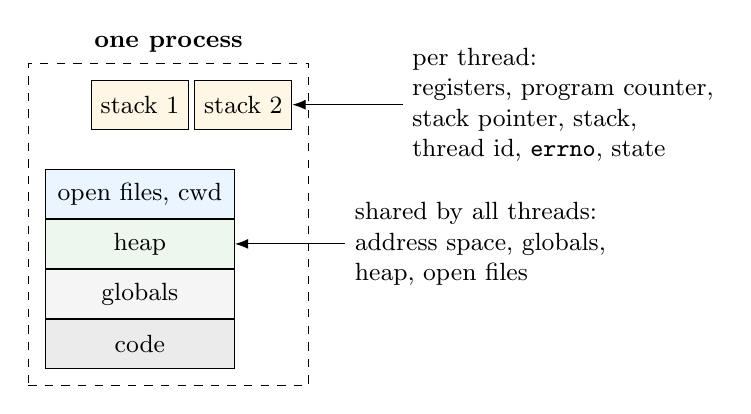
\begin{tikzpicture}[font=\small,
    box/.style={draw,minimum width=2.4cm,minimum height=0.62cm,align=center}]
  \node[box,fill=black!8] (code) {code};
  \node[box,fill=black!4,above=0pt of code] (data) {globals};
  \node[box,fill=keybg,above=0pt of data] (heap) {heap};
  \node[box,fill=newbg,above=0pt of heap] (files) {open files, cwd};
  \node[box,fill=warnbg,above=0.5cm of files,minimum width=1.1cm] (s1) {stack 1};
  \node[box,fill=warnbg,right=2pt of s1,minimum width=1.1cm] (s2) {stack 2};
  \node[draw,dashed,inner sep=6pt,fit=(code)(s1)(s2),
        label={[font=\small\bfseries]above:one process}] {};
  \node[right=1.4cm of s2,align=left] (r) {per thread:\\ registers, program counter,\\ stack pointer, stack,\\ thread id, \code{errno}, state};
  \draw[-Latex] (r.west) -- (s2.east);
  \node[right=1.4cm of heap,align=left] (sh) {shared by all threads:\\ address space, globals,\\ heap, open files};
  \draw[-Latex] (sh.west) -- (heap.east);
\end{tikzpicture}
\caption{Two threads in one process.}
\label{fig:threads}
\end{figure}

Everything reachable through a pointer is shared --- including another
thread's stack, if somebody hands out the address of a local variable.
``Private'' only means ``not shared unless you share it''.

\paragraph{Thread vs.\ process.} Creating a thread is much cheaper than
creating a process: no new address space, no copied page tables, no
copied descriptor table. Switching between threads of the same process
does not change the page tables either. The price: no isolation. One
thread's stray write corrupts every other thread, one thread's crash kills
the whole process, and every shared variable needs synchronisation
(chapters 3--5).

\section{The pthreads interface}

\begin{lstlisting}
int  pthread_create(pthread_t *thread, const pthread_attr_t *attr,
                    void *(*start_routine)(void *), void *arg);
void pthread_exit(void *retval);                 /* never returns */
int  pthread_join(pthread_t thread, void **retval);
int  pthread_detach(pthread_t thread);
pthread_t pthread_self(void);
\end{lstlisting}

\begin{description}
  \item[create] starts \code{start\_routine(arg)} in a new thread and
    stores its id in \code{*thread}. The new thread may run before or
    after \code{pthread\_create} returns --- never rely on either.
  \item[exit] ends the calling thread with a return value. Returning from
    \code{start\_routine} does the same. Returning from \code{main} (or
    calling \code{exit}) ends the \emph{whole process}, all threads
    included.
  \item[join] waits until the thread has ended and collects its return
    value. Afterwards the thread's resources are freed. Each thread can be
    joined once; joining yourself is an error (\code{EDEADLK}).
  \item[detach] ``nobody will join this thread'': its resources are freed
    as soon as it ends. A detached thread cannot be joined.
\end{description}

All functions return 0 or an error number (they do not set \code{errno}).

\section{The lifecycle}

A thread is created \emph{ready}, becomes \emph{running} when the
scheduler picks it, may \emph{block} (waiting for a lock, for I/O, in
\code{join}) and becomes ready again when woken, and finally
\emph{terminates}. A terminated thread that is joinable but not yet
joined is a \emph{zombie}: its stack can go, but its return value and id
must stay until somebody joins it --- exactly like a zombie process
(chapter~1). Neither joined nor detached means leaked: the zombie stays
forever. Chapter~10 builds this state machine.

\section{Passing arguments and results}

\paragraph{Arguments.} \code{arg} is a single \code{void *}. For more
than one value, pass a pointer to a struct --- and make sure the struct
lives long enough:

\begin{lstlisting}
struct job { int first, count; long result; };
struct job jobs[N];                      /* one per thread, in the caller's frame */
for (int i = 0; i < N; i++) {
  jobs[i] = (struct job){i * chunk, chunk, 0};
  pthread_create(&tid[i], NULL, worker, &jobs[i]);   /* not &i ! */
}
for (int i = 0; i < N; i++)
  pthread_join(tid[i], NULL);            /* jobs[] must outlive the threads */
\end{lstlisting}

Two classic bugs (\module{02}, part B): passing \code{\&i} (every thread
gets the same, changing address), and passing a pointer to a local of a
function that returns before the threads read it.

\paragraph{Results.} Either the thread writes into its own struct (as
above --- no sharing, no lock needed: each thread owns one element), or it
returns a pointer. Never return the address of a local; return heap
memory, a pointer into the argument, or a small integer cast to
\code{void *}.

\paragraph{Partition, then combine.} The simplest correct parallel
program splits the data into disjoint parts, lets each thread work only
on its part, and combines the partial results \emph{after}
\code{pthread\_join}. No shared writes, no locks --- and
\code{pthread\_join} guarantees that the joiner sees everything the
thread wrote (a happens-before edge, chapter~3).

\section{Thread-local data}

Some state must exist once per thread although it looks global. The
classic example is \code{errno}: if thread A's failing call and thread
B's failing call wrote the same variable, A could read B's error. C11 has
\code{\_Thread\_local} (GCC: \code{\_\_thread}); glibc keeps \code{errno}
in thread-local storage. \module{07}'s mini libc makes its
\code{ml\_errno} thread-local for exactly this reason.

\section{Who implements the threads?}

\begin{description}
  \item[Kernel-level threads (1:1).] Every user thread is a thread the
    kernel knows and schedules. Blocking in a system call blocks only that
    thread; threads run in parallel on several cores. Every switch goes
    through the kernel. Linux (NPTL), Windows --- and SWEB after A1.
  \item[User-level threads (M:1).] A library switches between threads
    inside one kernel thread (\module{10}). Switching is a function call,
    but a blocking system call blocks all threads, and only one core is
    used.
  \item[Hybrid (M:N).] M user threads on N kernel threads; complex and
    mostly abandoned (Go's runtime is a modern variant).
\end{description}

\begin{swebbox}
The stubs are in \file{userspace/libc/src/pthread.c}:
\code{pthread\_create} just \code{return -1;}. P1 turns it into a system
call that creates a new kernel \code{Thread} in the calling process
(1:1): it gets its own kernel stack (inside the \code{Thread} object,
\code{kernel\_stack\_}), its own user stack in the shared address space,
and its own saved registers --- and starts in user mode at a small libc
wrapper that calls \code{start\_routine(arg)} and then
\code{pthread\_exit} (chapter~10).
\end{swebbox}

\begin{keybox}
\begin{itemize}
  \item Threads share the address space and open files; each has its own
    registers and stack.
  \item Returning from the start routine = \code{pthread\_exit}; returning
    from \code{main} ends every thread.
  \item Join or detach every thread; an unjoined finished thread is a
    zombie.
  \item Pass each thread its own argument object that outlives it; never
    \code{\&i}, never a dying local.
  \item Partition-then-combine needs no locks; \code{join} makes the
    results visible.
\end{itemize}
\end{keybox}

\chapter{Race conditions}
\label{ch:races}

Two threads that only read shared data never disturb each other. As soon
as one of them writes, the result can depend on the exact order in which
the threads' instructions happen to interleave --- an order nobody
controls. This chapter explains why even \code{counter++} is not safe,
how to reason about interleavings, and which guarantees (``happens
before'') you can actually rely on.

\section{The lost update}

\code{counter++} looks like one step. The CPU executes three:

\begin{lstlisting}
mov  eax, [counter]     ; load
add  eax, 1             ; modify (in a register - private to the thread)
mov  [counter], eax     ; store
\end{lstlisting}

If thread A is interrupted (or simply runs on another core) between its
load and its store, both threads can load the same old value:

\begin{center}
\begin{tabular}{llc}
\toprule
\textbf{Thread A} & \textbf{Thread B} & \textbf{counter} \\
\midrule
load (reads 5)    &                    & 5 \\
                  & load (reads 5)     & 5 \\
                  & add, store 6       & 6 \\
add, store 6      &                    & \textbf{6} \\
\bottomrule
\end{tabular}
\end{center}

Two increments, one effect: a \emph{lost update}. Two threads with three
instructions each can interleave in $\binom{6}{3} = 20$ ways; only the 2
in which one thread's three instructions all come before the other's are
correct (\module{03}'s \code{interleave.c} lists all 20). With a million
increments per thread, the final count is usually far too small --- and
different in every run.

\section{Check-then-act}

A race needs no \code{++}. Any sequence ``look at shared state, then act
on what you saw'' breaks if the state changes in between:

\begin{lstlisting}
if (account->balance >= amount)        /* check */
  account->balance -= amount;          /* act: another thread may have
                                          withdrawn in between */
\end{lstlisting}

The same pattern appears as ``if the file does not exist, create it'',
``if the cache has no entry, compute and insert it'', ``if the pointer is
NULL, allocate''. In a kernel the dangerous variant is
\emph{time-of-check to time-of-use} (TOCTOU): the kernel checks a value in
user memory, then reads it again to use it --- and another user thread
changed it in between (chapter~7).

\section{Critical sections and atomicity}

A \emph{critical section} is a piece of code that accesses shared state
and must not run concurrently with other critical sections on the same
state. Making it \emph{atomic} means: every other thread sees either none
of its effects or all of them, never an intermediate state. There are
three ways to get there (\module{03}'s \code{three\_fixes.c} compares
them):

\begin{enumerate}
  \item \textbf{Lock it}: a mutex around the whole check-and-act
    (chapter~4).
  \item \textbf{Use an atomic operation}: \code{atomic\_fetch\_add} does
    load--add--store as one indivisible instruction (\code{lock xadd}).
    Only works when the whole critical section is a single such operation.
  \item \textbf{Do not share}: give each thread its own copy and combine
    afterwards (chapter~2's partition-then-combine).
\end{enumerate}

Invariants are the key to finding critical sections: ``the sum of all
balances is constant'', ``\code{count} equals the number of elements in
the list''. Every code path that temporarily breaks an invariant is a
critical section.

\section{Data race vs.\ race condition}

The two words are often mixed up:

\begin{description}
  \item[Data race] (a precise, mechanical definition): two threads access
    the same memory location, at least one access is a write, and the two
    accesses are not ordered by happens-before (no lock, no atomic, no
    join between them). In C and C++ a data race is \emph{undefined
    behaviour} --- the compiler may assume it never happens.
    ThreadSanitizer finds exactly these.
  \item[Race condition] (a semantic property): the program's correctness
    depends on timing. A program can have a race condition without a data
    race (every access is locked, but the lock is released between check
    and act) and a data race without visible harm (a statistics counter
    that may be a little off --- still undefined behaviour).
\end{description}

\section{Happens-before}

Which writes of thread A is thread B guaranteed to see? Only those that
\emph{happen before} B's read, where happens-before is built from:

\begin{itemize}
  \item program order within one thread;
  \item unlocking a mutex happens before the next lock of the same mutex;
  \item \code{pthread\_create} happens before the first instruction of the
    new thread; the thread's last instruction happens before
    \code{pthread\_join} returns;
  \item a release store to an atomic happens before an acquire load that
    reads it (chapter~4);
  \item transitivity: A before B and B before C gives A before C.
\end{itemize}

Anything else is unordered, and without an ordering there is no
guarantee at all --- not even that B ever sees A's write. The compiler
may keep a variable in a register for the whole loop:

\begin{lstlisting}
while (!done) {}       /* with a plain `int done`, -O2 may turn this into
                          `if (!done) for (;;);` - it never re-reads it */
\end{lstlisting}

and the CPU may make stores visible to other cores in a different order
than the program wrote them (chapter~4). \code{volatile} stops the
compiler from caching, but orders nothing between threads; use atomics or
locks.

\section{Why testing is not enough}

A race that loses one update in a million runs passes every normal test.
It also depends on the machine: more cores, a different load, an
optimised build or an extra \code{printf} change the timing. Hence the
modules test twice --- under ThreadSanitizer, which reports the data race
whenever the unordered accesses \emph{happen}, whether or not they
collide in that run, and optimised at full speed, where broken invariants
become visible.

\begin{swebbox}
SWEB is preemptive: the timer interrupt can switch threads at almost any
instruction, even in kernel code (\code{syscallHandler} enables
interrupts before calling \code{Syscall::syscallException}). After A1,
several threads of one process can be in the kernel at the same time,
touching the same process structures --- the thread list, the address
space, the file descriptors. Every such structure needs a lock, and every
``check, then act'' in your \code{pthread\_join} (``is the thread
finished? if not, sleep'') is a critical section. The A1 plan says it
bluntly: \emph{races appear on the tenth run, not the first.}
\end{swebbox}

\begin{keybox}
\begin{itemize}
  \item \code{x++} is load--modify--store; interleavings lose updates.
  \item Check-then-act is a race even without arithmetic; in the kernel
    it is TOCTOU.
  \item Find critical sections through invariants; fix them by locking,
    atomics, or not sharing.
  \item Data race = unordered conflicting accesses (undefined behaviour);
    race condition = timing-dependent correctness.
  \item Only happens-before edges (locks, create/join, atomics) guarantee
    visibility; \code{volatile} is not synchronisation.
\end{itemize}
\end{keybox}

\chapter{Locks from the hardware up}
\label{ch:locks}

A lock turns a critical section into something atomic. But how do you
build a lock if every load and store can be interleaved with those of
other threads? This chapter answers it from the bottom: the requirements,
the one-CPU trick (disable interrupts), a classic software algorithm that
fails on real hardware, the atomic instructions that make locks possible,
and the choice between spinning and sleeping --- which is exactly the
difference between SWEB's \code{SpinLock} and \code{Mutex}.

\section{What a lock must guarantee}

\begin{description}
  \item[Mutual exclusion] at most one thread in the critical section.
  \item[Progress] if the lock is free and threads want it, one of them
    gets it (no deadlock among the contenders).
  \item[Bounded waiting] a waiting thread gets its turn after a bounded
    number of others (no starvation) --- ``fairness''.
\end{description}
and in practice: cheap when uncontended, and not burning CPU time while
waiting for long.

\section{Disabling interrupts}

On a single CPU, the only way another thread can run in the middle of
your critical section is a timer interrupt that makes the scheduler
switch. Turn interrupts off (\code{cli}), do the work, turn them back on
(\code{sti}) --- nothing can interrupt you. This is how kernels protected
data before multi-core, and SWEB still uses it for the scheduler's own
data (\code{Scheduler::schedule} runs with interrupts off). But:
\begin{itemize}
  \item it is privileged --- user code cannot do it;
  \item it does not stop the \emph{other} cores on a multi-core machine;
  \item with interrupts off, timer ticks and device interrupts are
    delayed; the section must be very short, and must not sleep.
\end{itemize}

\section{Peterson's algorithm --- and why it breaks}

With only loads and stores, two threads can still achieve mutual
exclusion on paper:

\begin{lstlisting}
int flag[2], turn;                 /* shared */
void lock(int me) {
  int other = 1 - me;
  flag[me] = 1;                    /* I want in           */
  turn = other;                    /* but you go first    */
  while (flag[other] && turn == other) {}   /* wait while you want in and it's your turn */
}
void unlock(int me) { flag[me] = 0; }
\end{lstlisting}

It is correct under \emph{sequential consistency} --- the assumption that
all memory operations happen in one global order that respects each
thread's program order. Real CPUs do not guarantee that. On x86, a store
goes into the core's \emph{store buffer} and becomes visible to the other
core later; a subsequent load from a \emph{different} address can
overtake it. Both threads store their \code{flag}, both load the other's
still-old flag = 0 from memory, and both enter (\module{04}'s
\code{peterson.c} shows the violation within seconds). A \emph{memory
fence} (\code{mfence}, \code{atomic\_thread\_fence(memory\_order\_seq\_cst)})
between the stores and the loads repairs it. The lesson: correct
synchronisation needs help from the hardware.

\section{Atomic instructions}

\begin{description}
  \item[Test-and-set / exchange] \code{old = xchg(\&lock, 1)} writes 1 and
    returns the previous value, atomically. If \code{old} was 0, you have
    the lock. (\code{xchg} with memory is implicitly locked on x86.)
  \item[Compare-and-swap] \code{CAS(\&x, expected, new)}: if \code{x ==
    expected}, write \code{new} --- all at once --- and report success.
    The universal building block: any read-modify-write can be written as
    a CAS loop (\code{lock cmpxchg}).
  \item[Fetch-and-add] \code{old = fetch\_add(\&x, n)} (\code{lock xadd}):
    counters, and the ticket lock below.
\end{description}

C11 exposes them in \code{<stdatomic.h>}; GCC also has builtins such as
\code{\_\_sync\_lock\_test\_and\_set}, which SWEB uses.

\section{Spinlocks}

\begin{lstlisting}
void spin_lock(atomic_int *l) {
  for (;;) {
    if (!atomic_exchange(l, 1)) return;   /* test-and-set: got it */
    while (atomic_load(l)) {}             /* test: wait with plain reads */
  }
}
void spin_unlock(atomic_int *l) { atomic_store(l, 0); }
\end{lstlisting}

Waiting with plain reads (\emph{test-and-test-and-set}) matters: every
\code{xchg} needs exclusive ownership of the cache line, so a crowd of
cores hammering \code{xchg} keeps moving the line between them and slows
down even the lock holder. Reads can share the line until the holder's
unlock invalidates it.

A plain spinlock is unfair --- whoever happens to win the race gets it.
The \textbf{ticket lock} is FIFO: \code{my = fetch\_add(\&next, 1); while
(serving != my) \{\}}; unlock increments \code{serving}. Like a
deli-counter ticket.

\section{Spin or sleep?}

Spinning wastes the CPU for the whole wait. That is fine when the lock is
held for a few instructions and the holder is running on another core.
It is disastrous when the holder is \emph{not running} --- on a single
CPU the spinner burns its entire time slice while the holder cannot make
progress. Hence the three options:

\begin{enumerate}
  \item spin (short critical sections, multi-core, holder never sleeps);
  \item spin, but \code{yield} after a few tries (gives the holder a chance
    to run);
  \item \textbf{sleep}: put yourself on a wait queue, block, and let the
    unlocker wake you. Costs two context switches, wastes no CPU. Linux's
    \code{futex} makes the uncontended case a single atomic instruction in
    user space and enters the kernel only to sleep and wake.
\end{enumerate}

\section{Memory ordering in one paragraph}

Atomic operations also order the \emph{other} memory accesses around
them. Lock acquisition needs \emph{acquire} semantics (nothing from the
critical section may move before it), unlock needs \emph{release}
semantics (nothing may move after it). A release store paired with an
acquire load that reads it creates a happens-before edge (chapter~3).
C11's default, \code{memory\_order\_seq\_cst}, is the strongest and
simplest; use it unless you know exactly why a weaker order suffices.

\begin{swebbox}
\file{common/source/kernel/}: \code{SpinLock} tries
\code{ArchThreads::testSetLock} (an \code{xchg}); if the lock is taken it
records itself as waiting and loops \emph{test-and-set + yield} ---
spinning without yielding would be pointless on SWEB's single CPU.
\code{Mutex} sleeps instead: on contention it enqueues the thread in its
waiters list and calls \code{Scheduler::sleep()}; \code{release} pops a
waiter and wakes it. Both inherit from \code{Lock}, which keeps the
per-thread lists used for deadlock checks (chapter~6). User-space locks
in SWEB (\code{pthread\_spin\_*}, and mutexes that sleep only through a
small system call) are part of P1's elective.
\end{swebbox}

\begin{keybox}
\begin{itemize}
  \item Requirements: mutual exclusion, progress, bounded waiting.
  \item Disabling interrupts works only on one CPU and only in the kernel.
  \item Peterson needs sequential consistency; store buffers break it
    without fences.
  \item Locks are built from atomic read-modify-write instructions
    (xchg, CAS, fetch-and-add).
  \item Spin briefly, otherwise sleep; on one CPU never spin without
    yielding.
  \item Lock = acquire, unlock = release: that is what makes the data
    written inside visible to the next holder.
\end{itemize}
\end{keybox}

\chapter{Condition variables and semaphores}
\label{ch:condvars}

A mutex answers ``who may touch the data now?''. Threads also need to
\emph{wait for something}: for an element in a queue, for a thread to
finish, for the barber to wake up. Waiting correctly --- without burning
CPU and without missing the moment the condition becomes true --- is what
condition variables and semaphores are for. Your \code{pthread\_join} in
SWEB is one such wait; P1's elective asks for mutexes, condition variables
and semaphores in SWEB's user space.

\section{Waiting: spin or sleep}

\begin{lstlisting}
while (queue_empty(q)) {}          /* spinning: burns the CPU, and on one CPU
                                      the producer cannot even run */
\end{lstlisting}

Waiting should \emph{block}: take the thread off the CPU until another
thread says ``something changed''. Two problems must be solved together:
the waiter must not sleep through the signal (the \emph{lost wake-up}),
and the condition must be checked and the data accessed under a mutex.

\section{Condition variables}

\begin{lstlisting}
pthread_mutex_lock(&m);
while (!condition)                 /* ALWAYS a loop */
  pthread_cond_wait(&cv, &m);      /* atomically: unlock m and sleep;
                                      on wake-up: lock m again */
/* condition holds, and we hold m */
pthread_mutex_unlock(&m);

/* the other side */
pthread_mutex_lock(&m);
condition = true;
pthread_cond_signal(&cv);          /* wake one waiter (broadcast: all) */
pthread_mutex_unlock(&m);
\end{lstlisting}

A condition variable has no memory: a signal with nobody waiting is lost
--- by design. The \emph{condition} lives in ordinary shared variables,
protected by the mutex; the condition variable only provides ``sleep
until somebody might have changed it''.

\paragraph{Why \code{wait} must unlock atomically.} Suppose the waiter
unlocked, and only then went to sleep. In between, the signaller could
lock, set the condition, signal (nobody waits yet: lost) and unlock --- and
the waiter sleeps forever. \code{pthread\_cond\_wait} makes ``unlock and
sleep'' one step with respect to other threads. \module{05}'s
\code{lost\_wakeup.c} shows the broken and the fixed version.

\paragraph{Why \code{while}, not \code{if}.} Condition variables in
pthreads (and practically everywhere) have \emph{Mesa semantics}: a
signal only makes the waiter runnable; by the time it has re-acquired the
mutex, another thread may have consumed what it was woken for (a
\emph{stolen} wake-up). POSIX also allows \emph{spurious} wake-ups
without any signal. Rechecking in a loop handles both. (Under the
historical \emph{Hoare semantics} the signaller hands the mutex directly
to the woken thread, so the condition is guaranteed to hold --- simpler
to reason about, more expensive to implement.)

\paragraph{Signal or broadcast?} \code{signal} wakes one waiter: correct
when every waiter waits for the same thing and any one of them can
proceed. When waiters wait for different conditions on the same
variable, or when a change may allow several to proceed, use
\code{broadcast} --- a lost signal is a hang, an extra wake-up only costs
time.

\section{The bounded buffer}

The pattern to memorise (\module{05}, \code{bounded\_buffer.c}):

\begin{lstlisting}
void put(struct buf *b, int item) {
  pthread_mutex_lock(&b->m);
  while (b->count == CAP)
    pthread_cond_wait(&b->not_full, &b->m);
  b->item[(b->head + b->count++) % CAP] = item;
  pthread_cond_signal(&b->not_empty);
  pthread_mutex_unlock(&b->m);
}
int get(struct buf *b) {
  pthread_mutex_lock(&b->m);
  while (b->count == 0)
    pthread_cond_wait(&b->not_empty, &b->m);
  int item = b->item[b->head];
  b->head = (b->head + 1) % CAP;
  b->count--;
  pthread_cond_signal(&b->not_full);
  pthread_mutex_unlock(&b->m);
  return item;
}
\end{lstlisting}

\section{Semaphores}

Dijkstra's semaphore is a counter with two atomic operations:
\code{P} (\code{wait}, \code{sem\_wait}): wait until the value is
positive, then decrement; \code{V} (\code{signal}, \code{sem\_post}):
increment, waking a waiter if any. Unlike a condition variable, a
semaphore \emph{remembers}: a \code{post} with no waiter is kept in the
value. Three roles:

\begin{center}
\begin{tabular}{L{2.8cm}L{2cm}L{8.4cm}}
\toprule
\textbf{Role} & \textbf{Initial} & \textbf{Use} \\
\midrule
mutual exclusion & 1 & \code{wait}; critical section; \code{post} (a
``binary semaphore'' --- but anyone may \code{post}, unlike a mutex) \\
signalling & 0 & thread A \code{wait}s until thread B \code{post}s:
``B's event happened''; the order of the two calls does not matter \\
counting & $N$ & $N$ identical resources (buffer slots, connections) \\
\bottomrule
\end{tabular}
\end{center}

The bounded buffer with semaphores: \code{empty = CAP}, \code{full = 0},
\code{mutex = 1}; the producer does \code{wait(empty); wait(mutex); put;
post(mutex); post(full)}, the consumer the mirror image. The order of the
two \code{wait}s matters: \code{wait(mutex)} first and then blocking on
\code{empty} while holding it deadlocks the consumer.

A semaphore is easily built from a mutex and a condition variable
(\module{05}, part A) --- and conversely; they are equally powerful.

\section{Classic problems}

\paragraph{Readers--writers.} Many readers may read at once, a writer
needs exclusive access. The simple solution (readers count themselves;
the first reader locks writers out, the last one lets them in) lets a
steady stream of readers \emph{starve} writers. A writer-preferring lock
makes new readers wait as soon as a writer is waiting (\module{05},
part~B); a fair lock queues everybody in arrival order.

\paragraph{Sleeping barber.} A barber sleeps when there are no customers;
a customer wakes him, or waits in one of $N$ chairs, or leaves when all
chairs are taken. It combines signalling (customer wakes barber, barber
calls customer) with a counted resource (chairs) and needs care at the
edges: a customer arriving just as the barber decides to sleep must not
be lost, and shutdown must wake a sleeping barber (\module{05}, part~C).

\paragraph{Monitors.} A monitor bundles data, a mutex that every
operation holds, and condition variables --- the ``one object, one lock''
discipline as a language feature (Java's \code{synchronized} with
\code{wait}/\code{notify}). The bounded buffer above is a monitor written
by hand.

\begin{swebbox}
SWEB's \code{Condition} (\file{common/source/kernel/Condition.cpp}) is a
Mesa condition variable bound to a \code{Mutex}. \code{wait} puts the
thread on the waiters list \emph{while holding the list's lock}, releases
the mutex, and sleeps. The gap between unlocking the list and
\code{Scheduler::sleep()} is closed from the other side:
\code{Scheduler::wake} yields until the thread really is
\code{Sleeping} before it sets it \code{Running} --- no lost wake-up.
\code{Condition::wait} also asserts that the thread holds no other lock
while it sleeps. For \code{pthread\_join}: the joiner checks ``is the
thread finished?'' and waits on such a condition, under the lock that the
exiting thread takes to set ``finished'' and signal.
\end{swebbox}

\begin{keybox}
\begin{itemize}
  \item Wait by blocking; the condition lives in shared variables under a
    mutex.
  \item \code{cond\_wait} unlocks and sleeps atomically --- that is what
    prevents the lost wake-up.
  \item Always \code{while (!condition) wait}: Mesa semantics, stolen and
    spurious wake-ups.
  \item When unsure, \code{broadcast}.
  \item Semaphores remember posts: mutex (1), signal (0), count ($N$).
  \item Readers--writers: watch for writer starvation; barber: watch the
    edges and the shutdown.
\end{itemize}
\end{keybox}

\chapter{Deadlocks}
\label{ch:deadlocks}

Locks fix races and create the next problem: threads that wait for each
other forever. With two teams adding locks to shared SWEB structures ---
the thread list, the address space, the scheduler --- your group has to
agree on how locks are taken. This chapter gives the theory (Coffman's
conditions, graphs, prevention, avoidance, detection) and the practice
(lock ordering, validators), plus the relatives of deadlock: livelock,
starvation and priority inversion.

\section{Definition and the four conditions}

A set of threads is \emph{deadlocked} if every thread in the set waits
for an event that only another thread in the set can cause. The smallest
example: thread 1 holds lock A and waits for B, thread 2 holds B and waits
for A. A deadlock is possible only if all four \emph{Coffman conditions}
hold:

\begin{enumerate}
  \item \textbf{Mutual exclusion}: a resource is held by at most one
    thread.
  \item \textbf{Hold and wait}: a thread holds resources while waiting for
    more.
  \item \textbf{No preemption}: resources cannot be taken away; the holder
    releases them voluntarily.
  \item \textbf{Circular wait}: a cycle T$_1$ $\to$ T$_2$ $\to$ \dots $\to$
    T$_1$, each waiting for a resource the next one holds.
\end{enumerate}

Break any one and deadlock becomes impossible.

\section{Resource-allocation and wait-for graphs}

Draw threads as circles and resources as squares; an edge resource
$\to$ thread means ``held by'', thread $\to$ resource means ``waits
for''. With one instance per resource, a \emph{cycle means deadlock}.
Collapsing the resources gives the \emph{wait-for graph}: T$_i$ $\to$
T$_j$ if T$_i$ waits for something T$_j$ holds.

\begin{figure}[htbp]
\centering
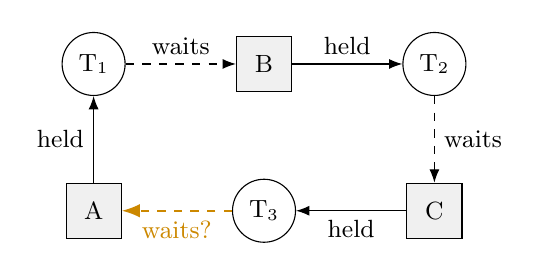
\begin{tikzpicture}[font=\small,node distance=1.4cm,
    t/.style={circle,draw,minimum size=0.8cm},
    r/.style={rectangle,draw,minimum size=0.7cm,fill=black!6},
    >=Latex]
  \node[t] (t1) {T$_1$};
  \node[r,right=of t1] (b) {B};
  \node[t,right=of b] (t2) {T$_2$};
  \node[r,below=1.1cm of t2] (c) {C};
  \node[t,left=of c] (t3) {T$_3$};
  \node[r,below=1.1cm of t1] (a) {A};
  \draw[->] (a) -- node[left] {held} (t1);
  \draw[->,dashed] (t1) -- node[above] {waits} (b);
  \draw[->] (b) -- node[above] {held} (t2);
  \draw[->,dashed] (t2) -- node[right] {waits} (c);
  \draw[->] (c) -- node[below] {held} (t3);
  \draw[->,dashed,warnrule,thick] (t3) -- node[below] {waits?} (a);
\end{tikzpicture}
\caption{T$_1$ holds A and waits for B, T$_2$ holds B and waits for C, T$_3$
holds C. No cycle: T$_3$ can finish. If T$_3$ now requests A, the cycle
T$_1\to$T$_2\to$T$_3\to$T$_1$ closes: deadlock.}
\label{fig:rag}
\end{figure}

\section{Strategies}

\paragraph{Prevention} --- make one condition impossible:
\begin{itemize}
  \item mutual exclusion: share instead (read-only data, lock-free
    structures) --- only for some resources;
  \item hold and wait: acquire everything at once, or release everything
    before waiting (trylock and back off --- risks livelock);
  \item no preemption: take resources away (roll back a transaction) ---
    rarely possible for locks;
  \item circular wait: \textbf{a global lock order}. If every thread takes
    locks in the same order, no cycle can form. This is the standard
    technique in kernels.
\end{itemize}

\paragraph{Avoidance} --- grant a request only if the system stays in a
\emph{safe state}: one from which some order lets every thread finish,
even if all of them ask for their declared maximum. The \emph{banker's
algorithm} checks this. Example with two resource types A (10 units) and
B (5 units):

\begin{center}
\begin{tabular}{lccc}
\toprule
 & \textbf{Allocation} & \textbf{Max} & \textbf{Need = Max -- Alloc} \\
\midrule
P$_0$ & (2, 1) & (7, 3) & (5, 2) \\
P$_1$ & (3, 1) & (4, 2) & (1, 1) \\
P$_2$ & (2, 2) & (5, 4) & (3, 2) \\
\bottomrule
\end{tabular}
\end{center}

Available = (10, 5) -- (7, 4) = (3, 1). Safety check: P$_1$'s need (1, 1)
$\le$ (3, 1): it can finish and return its allocation, Work = (6, 2);
then P$_2$ (3, 2) $\le$ (6, 2), Work = (8, 4); then P$_0$ (5, 2). Safe,
sequence P$_1$, P$_2$, P$_0$.
\begin{itemize}
  \item P$_0$ requests (1, 0): pretend to grant, Available = (2, 1), P$_0$'s
    need (4, 2). P$_1$, then P$_2$, then P$_0$ can still finish: safe,
    grant.
  \item P$_2$ requests (1, 1) instead: Available would be (2, 0). No
    thread's need fits into (2, 0) --- unsafe: P$_2$ must wait, although
    the units are free.
\end{itemize}
Avoidance needs to know maximum demands in advance; general-purpose
kernels therefore rarely use it, but it is a classic exam topic.

\paragraph{Detection and recovery} --- let deadlocks happen, find the
cycle in the wait-for graph, and break it (kill a thread, roll back).
Databases do this. A kernel can at least \emph{report} a deadlock instead
of hanging silently.

\paragraph{Ignore it} --- the ``ostrich algorithm''. For locks inside a
kernel, the real answer is prevention by lock ordering, backed by tools
that check the ordering.

\section{Lock ordering in practice}

\begin{itemize}
  \item Document a hierarchy: ``process lock before thread lock before
    address-space lock''. Code that holds a lower lock never acquires a
    higher one.
  \item Same-level locks (two accounts, two threads): order by a key ---
    the account number, the address of the lock object.
  \item Never call out into unknown code (callbacks, other subsystems)
    while holding a lock; you do not know which locks it takes.
  \item Keep critical sections small, and never sleep while holding a lock
    somebody else needs to wake you.
\end{itemize}

\paragraph{Validators.} Deadlocks depend on timing, tests rarely hit
them. A \emph{lock-order validator} records ``A was held while B was
acquired'' edges during a normal run and reports a cycle as soon as some
code path takes B then A --- even if the deadlock never happened. Linux
calls it \emph{lockdep}; ThreadSanitizer has one built in; \module{06},
part C builds one.

\section{Relatives of deadlock}

\begin{description}
  \item[Livelock] threads keep running but make no progress --- two
    threads that each trylock, fail, back off and retry in lockstep.
    Randomised back-off breaks the symmetry.
  \item[Starvation] the system makes progress, but one thread never gets
    its turn: an unfair lock, a reader-preferring rwlock, a low priority
    under strict priority scheduling (chapter~9).
  \item[Priority inversion] a high-priority thread waits for a lock held
    by a low-priority thread, while a medium-priority thread (which needs
    no lock) keeps the low one from running. The high thread effectively
    waits for the medium one. Mars Pathfinder (1997) reset itself because
    of this. \emph{Priority inheritance}: the lock holder temporarily
    runs with the priority of its highest waiter.
\end{description}

\begin{swebbox}
Every \code{Lock} knows its holder (\code{held\_by\_}); every
\code{Thread} keeps the locks it holds (\code{holding\_lock\_list\_}) and
the lock it waits for (\code{lock\_waiting\_on\_}). Before a thread goes
to sleep on a lock, \code{doChecksBeforeWaiting} can walk ``waits for lock
held by thread that waits for \dots'' and detect a real deadlock, and it
catches recursive locking. \code{\~{}Thread} asserts that a dying thread
holds no locks. Interrupt handlers must not take ordinary locks at all:
a handler waiting for a lock held by the thread it interrupted waits
forever --- a deadlock with a single thread.
\end{swebbox}

\begin{keybox}
\begin{itemize}
  \item Deadlock needs all four Coffman conditions; break one.
  \item Single-instance resources: a cycle in the wait-for graph is a
    deadlock.
  \item Kernels prevent deadlock with a documented lock order.
  \item Banker's algorithm: grant only if a safe sequence still exists.
  \item Validators find potential deadlocks from one run; SWEB's lock
    lists support similar checks.
  \item Livelock, starvation and priority inversion are the neighbours to
    recognise.
\end{itemize}
\end{keybox}

\chapter{System calls and user pointers}
\label{ch:syscalls}

User programs cannot touch devices, other processes or the kernel's
memory; the CPU refuses. Everything they need from outside their own
address space, they must \emph{ask} for --- through a system call, a
controlled door into the kernel. Your \code{pthread\_create} is such a
door, and every argument that comes through it is chosen by the user
program: possibly wrong, possibly malicious.

\section{User mode and kernel mode}

x86 CPUs run in one of four privilege levels (rings); operating systems
use two. In \emph{kernel mode} (ring~0) every instruction is allowed. In
\emph{user mode} (ring~3) privileged instructions --- \code{cli},
loading \code{cr3}, I/O ports --- raise an exception, and pages whose
page-table entries lack the \emph{user} bit are inaccessible
(chapter~8). The only ways from user to kernel mode are:

\begin{description}
  \item[Interrupts] from devices (timer, keyboard) --- asynchronous, not
    caused by the running code;
  \item[Exceptions] caused by the current instruction: page fault,
    division by zero, general protection fault;
  \item[Traps] deliberate: the program executes \code{int~n} or
    \code{syscall} to request a service.
\end{description}

All three enter the kernel at an address the kernel registered in advance
(the \emph{interrupt descriptor table}, or the \code{syscall} MSRs). The
program chooses \emph{which} service --- by a number --- never \emph{where}
the kernel starts executing. An interrupt gate also has a privilege level
(DPL): user code may only trigger gates with DPL~3 via \code{int~n}.

\section{Calling conventions}

\begin{center}
\begin{tabular}{L{2.4cm}L{3.2cm}L{4.4cm}L{3.2cm}}
\toprule
 & \textbf{Instruction} & \textbf{Number / arguments} & \textbf{Result} \\
\midrule
Linux x86-64 & \code{syscall} & \code{rax} / \code{rdi, rsi, rdx, r10, r8, r9}
& \code{rax}, errors as $-$errno \\
SWEB x86-64 & \code{int \$0x80} & \code{rax} / \code{rbx, rcx, rdx, rsi, rdi}
& \code{rax} \\
\bottomrule
\end{tabular}
\end{center}

Linux uses \code{r10} for the fourth argument because the \code{syscall}
instruction itself overwrites \code{rcx} (return address) and \code{r11}
(flags). SWEB passes the number plus five arguments --- exactly enough for
\code{pthread\_create}'s four arguments plus the address of a start
wrapper.

\paragraph{Errors.} The Linux kernel returns $-$errno (a value between
$-4095$ and $-1$). The libc wrapper turns it into $-1$ and stores the
positive number in \code{errno}, a \emph{thread-local} variable
(chapter~2). Any other value, even a ``negative'' address, is a valid
result --- hence the test \code{(unsigned long)r > -4096UL}.

\section{One system call, end to end}

\begin{figure}[htbp]
\centering
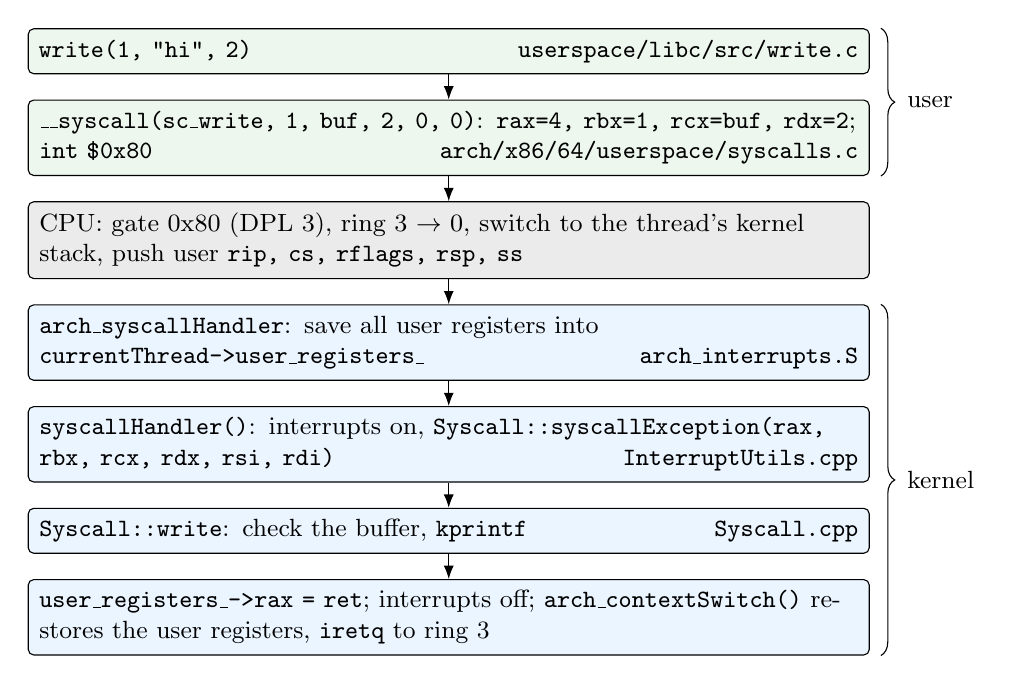
\begin{tikzpicture}[font=\small,node distance=0.32cm,
    s/.style={draw,rounded corners=2pt,align=left,inner sep=4pt,text width=10.4cm},
    >=Latex]
  \node[s,fill=keybg] (a) {\code{write(1, "hi", 2)} \hfill \file{userspace/libc/src/write.c}};
  \node[s,fill=keybg,below=of a] (b) {\code{\_\_syscall(sc\_write, 1, buf, 2, 0, 0)}: \code{rax=4, rbx=1, rcx=buf, rdx=2};
    \code{int \$0x80} \hfill \file{arch/x86/64/userspace/syscalls.c}};
  \node[s,fill=black!8,below=of b] (c) {CPU: gate 0x80 (DPL 3), ring 3 $\to$ 0, switch to the thread's kernel stack,
    push user \code{rip, cs, rflags, rsp, ss}};
  \node[s,fill=newbg,below=of c] (d) {\code{arch\_syscallHandler}: save all user registers into
    \code{currentThread->user\_registers\_} \hfill \file{arch\_interrupts.S}};
  \node[s,fill=newbg,below=of d] (e) {\code{syscallHandler()}: interrupts on,
    \code{Syscall::syscallException(rax, rbx, rcx, rdx, rsi, rdi)} \hfill \file{InterruptUtils.cpp}};
  \node[s,fill=newbg,below=of e] (f) {\code{Syscall::write}: check the buffer, \code{kprintf} \hfill \file{Syscall.cpp}};
  \node[s,fill=newbg,below=of f] (g) {\code{user\_registers\_->rax = ret}; interrupts off; \code{arch\_contextSwitch()}
    restores the user registers, \code{iretq} to ring 3};
  \foreach \x/\y in {a/b,b/c,c/d,d/e,e/f,f/g} \draw[->] (\x) -- (\y);
  \draw[decorate,decoration={brace,amplitude=5pt}] ([xshift=4pt]a.north east) -- ([xshift=4pt]b.south east)
    node[midway,right=6pt] {user};
  \draw[decorate,decoration={brace,amplitude=5pt}] ([xshift=4pt]d.north east) -- ([xshift=4pt]g.south east)
    node[midway,right=6pt] {kernel};
\end{tikzpicture}
\caption{The path of \code{write} through SWEB (x86-64).}
\label{fig:syscallpath}
\end{figure}

Note two details in figure~\ref{fig:syscallpath}. The kernel runs the
system call on the \emph{thread's own kernel stack}, so every thread needs
one (in SWEB it is part of the \code{Thread} object). And interrupts are
\emph{on} during the call: a system call can be preempted, and several
threads can be inside the kernel at once.

\section{Never trust a user pointer}

For \code{write(fd, buf, len)} the kernel reads \code{len} bytes at
\code{buf}. If it did so blindly, a program could pass a kernel address
and have the kernel copy kernel memory into a file --- or an unmapped
address and crash the kernel. Every pointer from user space must be
checked:

\begin{enumerate}
  \item \textbf{The whole range is user memory.} Not just the start:
    \code{buf + len} must also stay below the user/kernel boundary.
  \item \textbf{The check cannot overflow.} \code{buf + len > USER\_BREAK}
    fails when \code{buf + len} wraps around: \code{buf = 0x1000},
    \code{len = 0xfffffffffffff800} gives \code{0x800}, ``below the
    break''. Never add two user-controlled numbers; subtract from a
    constant:
\begin{lstlisting}
if (len > USER_BREAK || buf > USER_BREAK - len) return -EFAULT;
\end{lstlisting}
  \item \textbf{The pages exist} (or the kernel handles the fault on a bad
    user page without dying). Linux copies with \code{copy\_from\_user},
    which turns a fault into $-$\code{EFAULT}; SWEB's page-fault handler
    loads valid user pages on demand and ends the process otherwise.
  \item \textbf{Output buffers are writable.}
  \item \textbf{Strings} have no known length: copy byte by byte (page by
    page) into a bounded kernel buffer, checking each page as the copy
    reaches it --- \code{strlen} on a user pointer \emph{is} the unchecked
    read.
\end{enumerate}

Not everything that looks like a pointer is one. \code{pthread\_create}'s
\code{arg} is never dereferenced by the kernel --- it is passed to the new
thread --- so it must \emph{not} be checked; NULL and 42 are legal.
\code{start\_routine} is not dereferenced either; it becomes an
instruction pointer and at most needs to lie below \code{USER\_BREAK}.

\section{TOCTOU and the double fetch}

Once a process has several threads, user memory can change \emph{while}
the kernel works with it. If the kernel reads a value from user memory to
check it and reads it again to use it, another thread can swap it in
between:

\begin{lstlisting}
if (!access_ok(iov[i].base, iov[i].len)) return -EFAULT;   /* fetch 1 */
copy_to_device(iov[i].base, iov[i].len);                   /* fetch 2: may differ! */
\end{lstlisting}

The fix is simple and absolute: copy the user data into kernel memory
\emph{once}, then check and use only the copy. (Modern CPUs add SMAP, which
makes the kernel fault on any user-memory access outside explicit
copy routines.)

\begin{swebbox}
Syscall numbers live in \file{common/include/kernel/syscall-definitions.h},
shared by the kernel and the libc. Adding a system call means: a number,
a \code{case} in \code{Syscall::syscallException}, a static
\code{Syscall} method, and a libc wrapper calling \code{\_\_syscall}
(\module{11}, part 5 does it for \code{gettid}). SWEB's own checks are
the hand-written \code{buffer + size > USER\_BREAK} kind --- including the
overflow hole above. Your \code{pthread\_create} and \code{pthread\_join}
receive user pointers (\code{pthread\_t *}, \code{void **}); check them
properly, and check them \emph{before} you create or free anything.
\end{swebbox}

\begin{keybox}
\begin{itemize}
  \item The user picks the service number, never the kernel entry point;
    gates and privilege levels enforce it.
  \item Linux: \code{syscall}, args in \code{rdi rsi rdx r10 r8 r9},
    $-$errno; SWEB: \code{int \$0x80}, number in \code{rax}, args in
    \code{rbx rcx rdx rsi rdi}.
  \item Every system call runs on the calling thread's kernel stack, with
    interrupts on.
  \item Validate the whole user range, overflow-free; copy strings with
    per-page checks; do not check opaque arguments.
  \item Fetch user data once; check and use the kernel copy.
\end{itemize}
\end{keybox}

\chapter{Virtual memory}
\label{ch:vm}

Every process believes it owns a huge, private address space starting at
0. In reality its pages are scattered over physical memory, many of them
are not there at all, and some are shared with other processes. The MMU
translates every single memory access, and the kernel keeps the
translation tables. This chapter covers the translation (x86-64's
four-level page tables, the TLB), the page fault as the kernel's hook
into it (demand paging, copy-on-write), and what happens when physical
memory runs out (page replacement).

\section{Why virtual memory}

\begin{itemize}
  \item \textbf{Isolation}: a process can only reach the frames its page
    tables map; the kernel's pages are mapped without the user bit.
  \item \textbf{Relocation}: every program can be linked for the same
    addresses.
  \item \textbf{Overcommit}: memory is promised (\code{mmap} of 1~GiB) and
    delivered page by page on first touch; unused parts cost nothing.
  \item \textbf{Sharing}: the same physical frame can appear in several
    address spaces (shared libraries, copy-on-write after \code{fork}).
\end{itemize}

\section{Paging and the x86-64 page tables}

Memory is divided into 4~KiB \emph{pages} (virtual) and \emph{frames}
(physical). A page table maps page numbers to frame numbers. A flat table
for a 48-bit address space would have $2^{36}$ entries of 8 bytes ---
512~GiB per process. Instead, x86-64 uses a tree of four levels; each
table is one 4~KiB frame with 512 entries, and only the parts of the tree
that map something exist.

\begin{figure}[htbp]
\centering
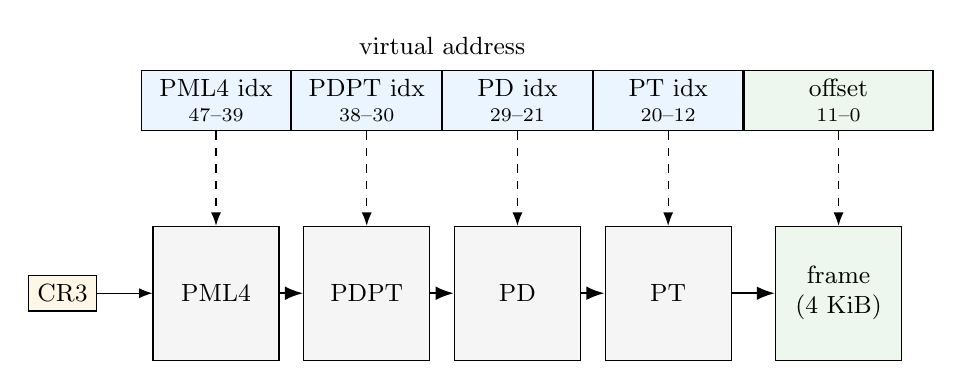
\begin{tikzpicture}[font=\small,>=Latex,
    f/.style={draw,minimum height=0.6cm,align=center},
    tab/.style={draw,minimum width=1.6cm,minimum height=1.7cm,fill=black!4,align=center}]
  % virtual address fields
  \node[f,minimum width=1.9cm,fill=newbg] (i4) {PML4 idx\\[-2pt]\scriptsize 47--39};
  \node[f,minimum width=1.9cm,fill=newbg,right=0pt of i4] (i3) {PDPT idx\\[-2pt]\scriptsize 38--30};
  \node[f,minimum width=1.9cm,fill=newbg,right=0pt of i3] (i2) {PD idx\\[-2pt]\scriptsize 29--21};
  \node[f,minimum width=1.9cm,fill=newbg,right=0pt of i2] (i1) {PT idx\\[-2pt]\scriptsize 20--12};
  \node[f,minimum width=2.4cm,fill=keybg,right=0pt of i1] (off) {offset\\[-2pt]\scriptsize 11--0};
  \node[above=2pt of i3.north east] {virtual address};
  % tables
  \node[tab,below=1.2cm of i4] (t4) {PML4};
  \node[tab,below=1.2cm of i3] (t3) {PDPT};
  \node[tab,below=1.2cm of i2] (t2) {PD};
  \node[tab,below=1.2cm of i1] (t1) {PT};
  \node[tab,below=1.2cm of off,fill=keybg] (fr) {frame\\(4 KiB)};
  \node[left=0.7cm of t4,draw,fill=warnbg] (cr3) {CR3};
  \draw[->] (cr3) -- (t4);
  \foreach \i/\t in {i4/t4,i3/t3,i2/t2,i1/t1,off/fr} \draw[->,dashed] (\i) -- (\t);
  \draw[->,thick] (t4) -- (t3); \draw[->,thick] (t3) -- (t2);
  \draw[->,thick] (t2) -- (t1); \draw[->,thick] (t1) -- (fr);
\end{tikzpicture}
\caption{A page walk: each 9-bit index selects one of 512 entries; the
entry holds the frame number of the next table, and finally of the page.}
\label{fig:pagewalk}
\end{figure}

A page-table entry (64 bits) holds the frame number (bits 12--51) and
flags, among them:
\begin{center}
\begin{tabular}{lll}
\toprule
\textbf{Bit} & \textbf{Name} & \textbf{Meaning} \\
\midrule
0 & P (present) & the entry is valid; otherwise any access faults \\
1 & W (writable) & stores allowed \\
2 & U (user) & accessible from ring 3 \\
5 & A (accessed) & set by the MMU on every access \\
6 & D (dirty) & set by the MMU on every write \\
9--11 & available & ignored by the MMU, free for the OS (e.g.\ a COW mark) \\
63 & NX & no instruction fetch \\
\bottomrule
\end{tabular}
\end{center}

The effective rights are the AND over all four levels: the upper levels
are usually created permissive (P, W, U) and the leaf entry decides.
Mapping one page into an empty address space costs three new tables
(PDPT, PD, PT); unmapping should free tables that became empty.

\section{The TLB}

A page walk costs four extra memory accesses. The \emph{translation
lookaside buffer} caches recent translations (page number $\to$ frame,
rights) and makes almost all accesses hit. The TLB is not coherent with
the page tables: when the kernel changes or removes a present entry, it
must invalidate the cached copy (\code{invlpg addr}, or reload \code{cr3}
to drop everything). Forgetting it leaves the old translation usable ---
after an unmap, a program keeps reading a frame that may already belong to
someone else. Entries that were not present are never cached, so
\emph{adding} a mapping needs no invalidation. On multi-core machines
other CPUs may cache the translation too: a \emph{TLB shootdown} sends
them an interrupt to invalidate --- expensive, and batched by real
kernels.

\section{Page faults}

When the MMU cannot translate (not present) or the rights do not allow
the access (write to read-only, user access to kernel page), it raises a
page fault: the CPU stores the faulting address (x86: in \code{cr2}) and
an error code (present?, write?, user?) and enters the kernel's handler.
The handler decides:

\begin{itemize}
  \item legal but not loaded yet: allocate/load the page, map it, return
    --- the CPU \emph{re-executes} the faulting instruction;
  \item copy-on-write page written: copy it, map the copy writable, return;
  \item anything else: the program made a mistake --- signal
    \code{SIGSEGV} (Linux) or end the process (SWEB).
\end{itemize}

\paragraph{Demand paging.} Nothing is loaded before it is used. Code
and data are read from the executable on the first access; heap and stack
pages are allocated on first touch and \textbf{zero-filled} --- a frame
straight from the free pool may contain another process's data. On Linux
even reading an untouched anonymous page only maps a shared zero page.

\paragraph{Copy-on-write.} \code{fork} shares all frames between parent
and child and makes every writable page read-only in \emph{both}, with a
software ``COW'' mark. The first write from either side faults; the
handler copies the frame and maps the copy writable. If the frame has only
one user left (reference count 1), it simply becomes writable again. Note
that the parent's TLB may still hold writable entries for those pages ---
they must be invalidated, or the parent's writes land in the shared frame.

\section{Page replacement}

When no frame is free, a page must be evicted (written to swap if dirty)
to make room. Which one?

\begin{description}
  \item[OPT (Belady)] evict the page whose next use lies furthest in the
    future. Optimal, but needs the future; the yardstick for the others.
  \item[FIFO] evict the page loaded longest ago. Simple, often bad, and it
    suffers from \emph{Belady's anomaly}: more frames can cause more
    faults.
  \item[LRU] evict the page unused for the longest time. Good, but exact
    LRU needs a timestamp per access --- too expensive in hardware.
  \item[Clock (second chance)] approximates LRU with the accessed bit: a
    hand sweeps over the frames; a page with R = 1 gets its bit cleared
    and a second chance, the first page with R = 0 is evicted.
\end{description}

Worked example, reference string \code{7 0 1 2 0 3 0 4 2 3 0 3 2 1 2 0 1 7
0 1}, 3 frames: FIFO 15 faults, LRU 12, OPT 9, Clock 14. Belady's anomaly
with FIFO on \code{1 2 3 4 1 2 5 1 2 3 4 5}: 9 faults with 3 frames, 10
with 4. LRU and OPT are \emph{stack algorithms} --- the pages kept with $k$
frames are always a subset of those kept with $k+1$ --- and never show the
anomaly. (\module{08}, part C simulates all four with exact rules.)

\paragraph{Working set and thrashing.} The \emph{working set} is the set
of pages a process used in the recent past. If the working sets of all
running processes do not fit into memory, every process keeps faulting
out the pages the others need: the system is busy paging and does no
useful work --- \emph{thrashing}. The remedy is fewer processes in memory
(suspend some), not a faster disk.

\begin{swebbox}
\file{arch/x86/64/source/ArchMemory.cpp}: \code{mapPage} walks the four
levels and allocates missing tables (P, W, U on the upper levels);
\code{unmapPage} frees tables that became empty; frames come from
\code{PageManager::allocPPN}. The kernel reaches any frame through the
identity mapping at \code{IDENT\_MAPPING\_START}
(\code{getIdentAddressOfPPN}). Page faults go to
\file{common/source/mm/PageFaultHandler.cpp}; a valid user fault calls
\code{Loader::loadPage}, which only knows the ELF segments --- a fault
elsewhere, e.g.\ just below the single stack page, ends the process.
For P1 this matters twice: every new thread needs its own user stack
somewhere in the shared address space, and two threads of one process can
now fault at the same time --- \code{mapPage} has no lock of its own.
\end{swebbox}

\begin{keybox}
\begin{itemize}
  \item Four levels of 512-entry tables; the leaf decides the rights, the
    MMU ANDs all levels.
  \item Changing or removing a present PTE requires a TLB invalidation.
  \item Page faults are the kernel's hook: demand paging (zero-filled!),
    copy-on-write, or kill.
  \item COW: read-only + mark in both address spaces, copy on first write,
    no copy for the last user.
  \item OPT $\le$ LRU; FIFO shows Belady's anomaly; Clock approximates LRU
    with the accessed bit.
  \item Thrashing: working sets do not fit; reduce the load.
\end{itemize}
\end{keybox}

\chapter{Scheduling}
\label{ch:scheduling}

Whenever more threads are ready than there are CPUs, the scheduler
decides who runs --- at every timer interrupt, and whenever a thread
blocks, wakes up, yields or exits. This chapter covers the metrics, the
classic policies you will be asked to simulate by hand in the exam, how
real systems combine them, and the question that matters most for your
\code{pthread\_join}: should a waiting thread spin, yield, or sleep?

% \gantt{chart}: one box per character, '.' = idle
\newcommand{\gantt}[1]{%
\begin{tikzpicture}[x=0.52cm,y=0.5cm,font=\scriptsize]
  \def\t{0}%
  \foreach \c [count=\i from 0] in {#1} {%
    \ifx\c.\draw (\i,0) rectangle ++(1,1);%
    \else\draw[fill=newbg] (\i,0) rectangle ++(1,1) node[pos=0.5] {\c};\fi
    \node[below] at (\i,0) {\i};
  }%
\end{tikzpicture}}

\section{Bursts and metrics}

Threads alternate between \emph{CPU bursts} (computing) and \emph{I/O
bursts} (waiting for the disk, the network, the keyboard, a lock).
CPU-bound threads have long CPU bursts, I/O-bound (interactive) threads
short ones. For a job that arrives at time $a$, first runs at $s$ and
finishes at $f$ with total CPU time $b$:

\begin{center}
\begin{tabular}{lll}
\toprule
\textbf{Metric} & \textbf{Definition} & \textbf{Who cares} \\
\midrule
turnaround time & $f - a$ & batch jobs \\
waiting time & $f - a - b$ (time spent ready, not running) & fairness \\
response time & $s - a$ & interactive users \\
throughput & jobs finished per time unit & the whole system \\
\bottomrule
\end{tabular}
\end{center}

The goals conflict: short quanta improve response and cost throughput
(context switches); favouring short jobs improves the average and can
starve long ones.

\section{The classic policies}

Example (arrival, burst, priority): A (0, 5, 2), B (1, 3, 1), C (2, 1, 3),
D (4, 2, 1) --- \module{09}, question 1. One box per time unit.

\paragraph{FCFS} (first come, first served): run jobs to completion in
arrival order. Simple, no starvation, but short jobs wait behind long ones
--- the \emph{convoy effect}.

\begin{center}\gantt{A,A,A,A,A,B,B,B,C,D,D}\\ average waiting 3.75\end{center}

\paragraph{SJF} (shortest job first, non-preemptive): when the CPU becomes
free, pick the job with the shortest burst. When all jobs are present
from the start, this is provably optimal for the average waiting time
(exchange argument: a longer job directly in front of a shorter one ---
swap them, and the sum of waiting times drops). With staggered arrivals
it is only a good heuristic: a short job arriving just after a long one
has started still has to wait.

\begin{center}\gantt{A,A,A,A,A,C,D,D,B,B,B}\\ average waiting 3.00\end{center}

\paragraph{SRTF} (shortest remaining time first): SJF with preemption ---
a new job with less remaining work than the running one takes over.
Optimal for the average waiting time over all schedules.

\begin{center}\gantt{A,B,C,B,B,D,D,A,A,A,A}\\ average waiting 2.00, response 0.25\end{center}

Both need the length of the next CPU burst, which the OS does not know.
It can \emph{predict} it by exponential averaging of the past bursts:
$\tau_{n+1} = \alpha t_n + (1-\alpha)\tau_n$.

\paragraph{Round robin} (RR): a FIFO ready queue; each job runs for at
most one \emph{quantum} $q$, then goes to the end of the queue. Good
response time, fair, no starvation. The quantum is the knob: too small and
the CPU is busy switching (a 0.1~ms switch with $q$ = 1~ms wastes 9\%),
too large and RR degenerates into FCFS. Typical values: a few
milliseconds. With $q = 2$:

\begin{center}\gantt{A,A,B,B,C,A,A,D,D,B,A}\\ average waiting 4.25, response 1.50\end{center}

A tie that exams love: at $t = 2$, C arrives \emph{and} A's quantum
ends. The convention used in \module{09} (and by most textbooks): the
newcomer is queued first, the preempted job behind it. State your
convention when you answer.

\paragraph{Priority} scheduling: always run the most important ready job
(here: smaller number = more important; preemptive):

\begin{center}\gantt{A,B,B,B,D,D,A,A,A,A,C}\\ average waiting 3.25\end{center}

Low-priority jobs can \emph{starve} if higher-priority work keeps
arriving. Remedy: \emph{aging} --- raise the priority of waiting jobs over
time. Also watch for priority inversion (chapter~6).

\section{Multi-level feedback queue}

MLFQ learns what kind of job it deals with, without being told:

\begin{enumerate}
  \item Several queues with decreasing priority; round robin within a
    queue; higher queues always win, and preempt lower ones.
  \item A new job enters the top queue.
  \item A job that uses up its time allotment on a level is moved one
    level down. The allotment is counted \emph{across} I/O --- otherwise a
    job could stay on top by blocking just before its quantum ends.
  \item Periodically, all jobs are boosted back to the top: no
    starvation, and a job that changed its behaviour gets a new chance.
\end{enumerate}

Interactive jobs (short bursts) stay high and get quick responses;
CPU-bound jobs sink and share the rest. \module{09}'s bonus implements it
with exact rules.

\section{Proportional share and Linux}

Instead of priorities, give each job a \emph{share}: lottery scheduling
draws tickets, stride scheduling advances a ``pass'' value by
1/tickets. Linux's scheduler (CFS, since 6.6 EEVDF) is of this kind: each
task accumulates \emph{virtual runtime}, weighted by its nice value (nice
0 = weight 1024, each nice step $\approx$ 1.25$\times$ less), and the task
with the least virtual runtime runs next. A task that sleeps a lot has
little virtual runtime and runs soon after waking --- interactive tasks
stay responsive without explicit classification (\module{09}'s examples
measure both effects).

\section{Spin, yield or sleep?}

A thread that must wait for another thread (a flag, a lock, a join) on a
\emph{single} CPU:

\begin{description}
  \item[spin] (\code{while (!flag) \{\}}): burns its whole quantum every
    round --- and the flag cannot change meanwhile, because the thread
    that would set it is not running. Pure waste.
  \item[yield] (\code{while (!flag) yield();}): gives the CPU away at once,
    but stays \emph{runnable}: it is scheduled again and again just to
    check and yield. Costs a context switch per round, forever.
  \item[sleep] (block until woken): leaves the ready queue entirely; costs
    exactly one switch away and one back.
\end{description}

A kernel waits by sleeping, except for very short waits on locks held
for a few instructions.

\begin{swebbox}
\code{Scheduler::schedule()} (\file{common/source/kernel/Scheduler.cpp})
is round robin: it picks the first thread in \code{threads\_} that is
\code{Running} (i.e.\ schedulable) and rotates the list. The timer
interrupt (\code{irqHandler\_0}) calls it every tick, so the quantum is one
tick; \code{Scheduler::yield()} triggers the same code voluntarily with
\code{int \$65}. When nothing is runnable, the idle thread runs.
\code{sleep()} sets the state to \code{Sleeping}, which removes a thread
from consideration until \code{wake()} sets it back. For
\code{pthread\_join}: the joiner must \emph{sleep} until the target has
exited --- a \code{while (!done) yield();} loop would ``work'' and waste
every round-robin cycle.
\end{swebbox}

\begin{keybox}
\begin{itemize}
  \item Metrics: turnaround $f-a$, waiting $f-a-b$, response $s-a$.
  \item FCFS (convoys), SJF (optimal when all jobs start together), SRTF (optimal),
    RR (response; quantum trade-off), priority (starvation $\to$ aging).
  \item MLFQ: demote on used allotment (across I/O), boost periodically.
  \item Linux: weighted virtual runtime, nice changes the weight.
  \item Wait by sleeping; on one CPU, spinning is pointless and yielding
    in a loop is wasteful.
\end{itemize}
\end{keybox}

\chapter{Implementing threads}
\label{ch:impl}

Chapter~2 used threads; this chapter builds them. The mechanics are the
same whether the switching happens in a user-level library
(\module{10}) or in a kernel (SWEB): a record per thread, a way to save
and restore registers, a stack per thread, a state machine, and wait
queues. The hard parts are at the edges --- how a thread starts, how it
ends, who frees its stack, and what happens when an interrupt arrives in
the middle of the library's own bookkeeping.

\section{The thread control block and the context}

For each thread the implementation keeps a \emph{thread control block}
(TCB): id, state, saved registers (the \emph{context}), stack, start
routine and argument, return value, detached flag, and links for the
queues it may sit in.

A context switch saves the running thread's registers into its TCB and
loads the next thread's registers from its TCB. Loading the stack pointer
switches stacks; loading the instruction pointer continues wherever the
next thread stopped. From the thread's point of view, the call that
switched away simply returns --- later. \code{swapcontext(\&old, \&new)}
does exactly this in user space; SWEB's \code{arch\_contextSwitch}
restores a \code{Thread}'s saved \code{ArchThreadRegisters}.

\section{States}

\begin{figure}[htbp]
\centering
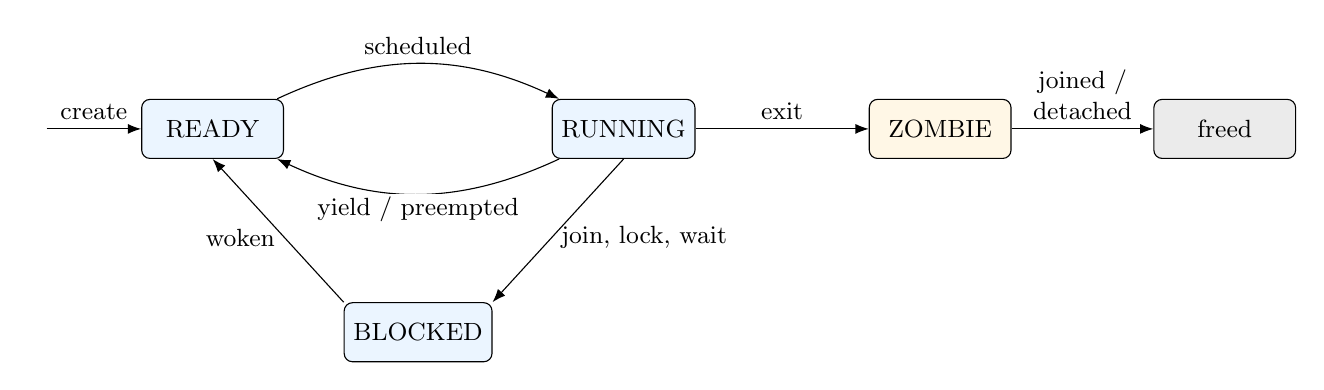
\begin{tikzpicture}[font=\small,>=Latex,node distance=3.4cm,
    st/.style={draw,rounded corners=3pt,minimum width=1.8cm,minimum height=0.75cm,fill=newbg}]
  \node[st] (ready) {READY};
  \node[st,right=of ready] (run) {RUNNING};
  \node[st,below=2.2cm of $(ready)!0.5!(run)$] (blk) {BLOCKED};
  \node[st,right=2.2cm of run,fill=warnbg] (zom) {ZOMBIE};
  \node[st,right=1.8cm of zom,fill=black!8] (free) {freed};
  \node[left=1.2cm of ready] (new) {};
  \draw[->] (new) -- node[above] {create} (ready);
  \draw[->] (ready) to[bend left=25] node[above] {scheduled} (run);
  \draw[->] (run) to[bend left=25] node[below,fill=white,inner sep=1pt] {yield / preempted} (ready);
  \draw[->] (run.south) -- node[right,pos=0.55] {join, lock, wait} (blk.north east);
  \draw[->] (blk.north west) -- node[left,pos=0.45] {woken} (ready.south);
  \draw[->] (run) -- node[above] {exit} (zom);
  \draw[->] (zom) -- node[above,align=center] {joined /\\detached} (free);
\end{tikzpicture}
\caption{Thread states. SWEB's names: \code{Running} covers READY and
RUNNING, \code{Sleeping} is BLOCKED, \code{ToBeDestroyed} is the way out.}
\label{fig:states}
\end{figure}

A BLOCKED thread is in no ready queue; exactly one wait queue (a mutex's,
a condition's, a joiner slot) knows it, and whoever makes the awaited
event happen moves it back to READY.

\section{Birth: a stack and a trampoline}

A new thread needs a stack of its own and a first context that ``returns''
into its code. The first instruction must not be the start routine itself:
when \code{start\_routine} returns, it would return to whatever garbage
lies on the fresh stack. Instead the thread starts in a small
\emph{trampoline}:

\begin{lstlisting}
static void trampoline(void) {
  after_switch();                                 /* see "Death" below */
  uthread_exit(current->start(current->arg));      /* return == exit */
}
\end{lstlisting}

Stacks should have a \emph{guard page} below them (mapped without any
access rights), so that an overflow faults at once instead of silently
overwriting the neighbouring stack.

\section{Death: exit, zombies, join, detach}

\begin{itemize}
  \item \textbf{exit}: store the return value, become a ZOMBIE, wake the
    joiner if one waits, switch away --- forever.
  \item \textbf{join}: if the target is already a zombie, collect and free
    it; otherwise block until its exit wakes you, then collect and free.
    Errors: no such thread (\code{ESRCH}), joining yourself or closing a
    cycle of joins (\code{EDEADLK}), a detached target or a second joiner
    (\code{EINVAL}).
  \item \textbf{detach}: nobody will join; free the thread as soon as it
    is a zombie (at once, if it already is).
\end{itemize}

\paragraph{Nobody frees their own stack.} A detached thread that exits
cannot unmap its stack --- it is still running on it; the next push or
return would fault. The freeing has to happen \emph{after} the switch, by
somebody else: \module{10}'s library notes the thread in a variable, and
the next thread to run frees it right after the switch (in
\code{after\_switch}, which the trampoline also calls). SWEB solves the
same problem for kernel stacks with a dedicated thread:
\code{Thread::kill} only marks the thread \code{ToBeDestroyed}, and the
cleanup thread \code{delete}s it later.

\section{Blocking primitives}

A blocking mutex is an owner plus a FIFO of waiting TCBs:
\begin{itemize}
  \item lock: free $\to$ take it; else enqueue yourself, state BLOCKED,
    switch away;
  \item unlock: waiters? either \emph{hand the mutex over} to the first
    one (FIFO, fair, but every contended unlock forces a switch) or free
    it and wake a waiter who must compete again (\emph{barging}: faster,
    unfair --- SWEB's \code{Mutex} does this).
\end{itemize}

A condition variable is just a wait queue; \code{wait} enqueues,
unlocks the mutex and blocks \emph{without any switch in between},
then re-locks after being woken. Deadlock detection comes almost for free:
if the ready queue is empty but some thread is BLOCKED, nothing can ever
wake it.

\section{Preemption and interrupt safety}

Without preemption, a thread runs until it calls into the library;
atomicity inside the library is automatic. With a timer
(\module{10}'s bonus uses \code{SIGVTALRM}, the kernel uses the timer
interrupt), a switch can happen \emph{anywhere} --- also in the middle of
\code{q\_push} or between ``mutex is free'' and ``I am the owner''. The
library's own data then needs protection: block the signal (user space)
or disable interrupts (kernel, one CPU) around every operation on it,
exactly as SWEB's scheduler runs with interrupts off. On several CPUs this
is not enough; a spinlock is needed as well.

And code that can be interrupted at any instruction must not be
re-entered through non-reentrant functions: a thread preempted inside
\code{malloc} holds malloc's lock; another thread on the same kernel
thread calling \code{malloc} deadlocks. SWEB's version of the rule: no
\code{new}/\code{delete} with interrupts off or in interrupt handlers.

\section{User-level vs.\ kernel-level, revisited}

\begin{center}
\begin{tabular}{L{3.6cm}L{4.8cm}L{4.8cm}}
\toprule
 & \textbf{User-level (M:1)} & \textbf{Kernel-level (1:1)} \\
\midrule
switch cost & function call + registers (\module{10}: $\approx$0.4 µs,
mostly glibc's signal-mask syscall) & kernel entry, scheduler, exit
($\approx$3 µs in \module{10}'s measurement) \\
blocking syscall & blocks \emph{all} threads & blocks only the caller \\
multiple cores & no & yes \\
per thread & TCB, user stack & kernel stack, user stack, two register
sets, kernel TCB \\
\bottomrule
\end{tabular}
\end{center}

\begin{swebbox}
After A1 every pthread is a kernel \code{Thread} (1:1). The pieces map
one to one:
\begin{itemize}
  \item TCB = \code{Thread}; its \code{kernel\_stack\_} is 8~KiB inside
    the object; \code{user\_registers\_} and \code{kernel\_registers\_} are
    the two contexts (user mode, and the kernel side of a system call or
    interrupt).
  \item Birth: \code{ArchThreads::createUserRegisters(regs, entry,
    user\_stack\_top, kernel\_stack)}; \code{entry} = a libc wrapper that
    calls \code{start\_routine(arg)} and then \code{pthread\_exit}; the two
    values reach it in \code{rdi}/\code{rsi}. \code{setAddressSpace} gives
    the thread the process's page tables.
  \item The user stack: a new region in the shared address space, below
    the first thread's stack page, with a guard gap (chapter~8).
  \item Death and reaping: \code{kill} $\to$ \code{ToBeDestroyed} $\to$
    cleanup thread. Join data (return value, finished) must survive the
    \code{Thread} object --- keep it in the process.
  \item Waiting: \code{Condition}/\code{Mutex} (chapter~5), never a yield
    loop (chapter~9).
\end{itemize}
\end{swebbox}

\begin{keybox}
\begin{itemize}
  \item A context switch = save registers into one TCB, load them from
    another; the stack pointer switches the stack.
  \item Start through a trampoline so that returning means exiting; guard
    pages catch stack overflows.
  \item Zombies keep the return value until join; detached threads are
    freed at exit --- by somebody else, after the switch.
  \item Blocking = a wait queue + state BLOCKED + switch; hand-off vs.
    barging.
  \item Preemption makes the library's own data shared: disable
    interrupts / block the signal; no non-reentrant calls.
\end{itemize}
\end{keybox}

\chapter{SWEB: putting it together}
\label{ch:sweb}

SWEB is the course's teaching kernel: small enough to read, real enough to
boot on x86-64 hardware (in QEMU). This last chapter is a map --- where
things are, how the machine gets from power-on to the shell, where each
idea of chapters 1--10 lives in the code --- and a guide to the A1 work:
what changes, and how to test it so that it survives the tenth run.
\module{11}'s worksheet walks through all of it with questions.

\section{The source tree}

\begin{center}
\begin{tabular}{L{5.4cm}L{8.4cm}}
\toprule
\textbf{Path} & \textbf{Contents} \\
\midrule
\file{common/source/kernel/} & \code{main.cpp} (\code{startup}), \code{Thread},
\code{UserProcess}, \code{Scheduler}, \code{Syscall}, \code{Loader},
\code{ProcessRegistry}, locks (\code{Lock}, \code{Mutex}, \code{SpinLock},
\code{Condition}), \code{CleanupThread}, \code{IdleThread} \\
\file{common/source/mm/} & \code{PageManager} (frames),
\code{KernelMemoryManager} (kernel heap), \code{PageFaultHandler} \\
\file{common/source/fs/}, \file{console/} & VFS, minix file system, terminal,
\code{kprintf} and \code{debug()} \\
\file{common/include/kernel/} & headers, \code{syscall-definitions.h} (numbers,
shared with the libc), \code{user\_progs.h} \\
\file{common/include/console/debug.h} & debug categories (switch
output on/off per category) \\
\file{arch/x86/64/} & page tables (\code{ArchMemory}), registers and context
switch (\code{ArchThreads}, \code{arch\_interrupts.S}), the IDT and all
interrupt handlers (\code{InterruptUtils.cpp}), \code{offsets.h}
(\code{USER\_BREAK}) \\
\file{userspace/libc/} & SWEB's own small C library: \code{write.c},
\code{pthread.c} (stubs), \code{nonstd.c} (\code{\_start}) \\
\file{userspace/tests/} & user programs; every \code{x.c} becomes
\code{x.sweb} on the disk image \\
\bottomrule
\end{tabular}
\end{center}

\section{From power-on to the shell}

\begin{enumerate}
  \item GRUB loads the kernel (the menu has no timeout --- press Enter);
    early assembly sets up paging and jumps to \code{startup()}.
  \item \code{startup()} creates the console, the scheduler (with the
    cleanup and idle threads), mounts the root file system and adds the
    \code{ProcessRegistry} thread; then it enables interrupts and yields ---
    from now on the scheduler runs everything.
  \item \code{ProcessRegistry::Run} mounts the user-program partition at
    \file{/usr} and creates a \code{UserProcess} for each entry of
    \code{user\_progs} --- by default only \file{/usr/shell.sweb}.
  \item The \code{UserProcess} constructor opens the binary, creates a
    \code{Loader} (reads the ELF headers), maps one stack page below
    \code{USER\_BREAK}, sets the user registers (\code{rip} = ELF entry =
    \code{\_start}, \code{rsp} = \code{USER\_BREAK - 8}) and the address
    space; the scheduler switches to it in user mode.
  \item Every first touch of code or data page-faults and is loaded by
    \code{Loader::loadPage}. The shell reads commands with \code{sc\_read}
    and starts programs with \code{createprocess}.
\end{enumerate}

\section{Every chapter in the code}

\begin{center}
\begin{tabular}{L{2.2cm}L{11.6cm}}
\toprule
\textbf{Chapter} & \textbf{Where in SWEB} \\
\midrule
1 processes & \code{UserProcess} (= a thread today), \code{ProcessRegistry},
\code{createprocess}; no \code{fork}/\code{exec} yet (Team F) \\
2 threads & \code{pthread.c} stubs; \code{Thread} with \code{kernel\_stack\_}
and two register sets \\
3 races & a preemptive kernel: interrupts are on during system calls \\
4 locks & \code{SpinLock} (test-and-set + yield), \code{Mutex} (sleeps),
\code{ArchThreads::testSetLock}, interrupts off in \code{schedule()} \\
5 condvars & \code{Condition}; \code{Scheduler::sleep}/\code{wake} with the
wait-until-sleeping loop \\
6 deadlocks & \code{holding\_lock\_list\_}, \code{lock\_waiting\_on\_},
\code{doChecksBeforeWaiting}; no locks in interrupt handlers \\
7 syscalls & \code{int \$0x80}, \code{arch\_syscallHandler},
\code{Syscall::syscallException}, \code{buffer + size > USER\_BREAK} checks \\
8 memory & \code{ArchMemory::mapPage/unmapPage}, \code{PageManager},
\code{PageFaultHandler}, \code{Loader::loadPage}, identity mapping \\
9 scheduling & round robin in \code{Scheduler::schedule}, one tick per quantum,
\code{yield} = \code{int \$65} \\
10 threads & \code{Thread} states, \code{kill} $\to$ \code{ToBeDestroyed} $\to$
cleanup thread \\
\bottomrule
\end{tabular}
\end{center}

\section{What A1 changes}

\paragraph{Phase 0 (all four, 1--4 Oct): split process from thread.} A
process owns the address space (\code{Loader}/\code{ArchMemory}), the file
descriptors and the PID; a thread owns its stacks, registers, state and
TID. Consequences to design together: how a thread finds its process
(a pointer; keeping \code{Thread::loader\_} as a non-owning shortcut
saves many edits), who destroys the process and when (after its
\emph{last} thread, in the cleanup thread --- never on a stack or in an
address space that is about to disappear), how ids are handed out (today
every \code{tid\_} is 0), and what \code{ProcessRegistry} counts.

\paragraph{Team P.} \code{pthread\_create} (P1): the system call, argument
checks, a new thread with its own user stack and a start wrapper.
\code{pthread\_exit} (P2): the return value survives the thread, the
stack is freed, the process keeps running. \code{pthread\_join} (P1): block
until the target has finished, receive exactly the stored value; a
detached thread cannot be joined. \code{pthread\_cancel} (P2): end the
target at a defined cancellation point.

\paragraph{Team F.} \code{fork} with copy-on-write, \code{exec} --- and,
together with Team P, their behaviour in multi-threaded processes
(\code{fork} duplicates only the calling thread; \code{exit} tears down
every thread).

\section{Testing}

The course grades with your own tests and with the Tacos test system;
neither replaces the other. Practical rules:

\begin{itemize}
  \item Write the test program first (\file{userspace/tests/}); re-run
    CMake after adding one, and build twice if the new program is missing
    from the image.
  \item Test the edges, not only the happy path: bad user pointers,
    joining yourself or twice, main exiting first, a thread creating
    threads, many threads, create/join in a loop (leaks).
  \item Run every test many times: \module{11}'s \code{sweb\_run.py -n 10}
    boots SWEB headless ten times and reports hangs (exit 1) and kernel
    panics (exit 2). Races appear on the tenth run.
  \item Use the debug categories (\code{debug.h}) instead of scattering
    \code{kprintf}; switch noisy ones off. For hard cases: \code{make
    qemugdb} + \code{make rungdb}.
  \item Assertions are cheap documentation: \code{assert(lock.isHeldBy(currentThread))}
    at the top of a function that needs the lock.
\end{itemize}

\section{Pitfalls that cost days}

\begin{itemize}
  \item \code{new}/\code{delete} with interrupts off or in a handler: the
    kernel-heap lock may be held by the interrupted thread.
  \item Sleeping while holding a lock the waker needs; \code{Condition::wait}
    asserts against extra held locks for a reason.
  \item Deleting a thread (or an address space) that is still running or
    still in use --- defer to the cleanup thread.
  \item Trusting user pointers, or checking them with an overflowing sum.
  \item Busy-waiting (\code{while (!done) yield();}) instead of sleeping on a
    condition.
  \item Two threads faulting on the same missing page table at once:
    \code{mapPage} needs a lock once a process has several threads.
  \item Checking once, using later (TOCTOU) --- in user memory and in
    kernel state: ``is the thread still alive?'' must be answered and acted
    on under the same lock.
\end{itemize}

\begin{keybox}
\begin{itemize}
  \item Know the map: \file{common/source/kernel}, \file{mm},
    \file{arch/x86/64}, \file{userspace/libc}, \file{userspace/tests}.
  \item Boot path: \code{startup} $\to$ \code{ProcessRegistry} $\to$
    \code{UserProcess} $\to$ lazy loading by page faults.
  \item A1 starts with the process/thread split --- agree on ownership,
    lifetime, ids and locking as a group.
  \item Test the edges, many times, headless; read the debug output.
\end{itemize}
\end{keybox}


\end{document}
